% !TEX root = ../OT4ML.tex

%%%%%%%%%%%%%%%%%%%%%%%%%%%%%%%%%%%%%%%%%%%%%%%%%%%%%%%%%%%%%%%%%%%%%%%%%%%
%%%%%%%%%%%%%%%%%%%%%%%%%%%%%%%%%%%%%%%%%%%%%%%%%%%%%%%%%%%%%%%%%%%%%%%%%%%
%%%%%%%%%%%%%%%%%%%%%%%%%%%%%%%%%%%%%%%%%%%%%%%%%%%%%%%%%%%%%%%%%%%%%%%%%%%
\chapter{Statistical Optimal Transport}
\label{sec-statistical-ot}
\index{statistical optimal transport}% strictindex
\index{empirical!measure}% strictindex
\index{sample complexity}% strictindex
\index{bias-variance tradeoff}% strictindex

Optimal transport is rarely evaluated on population measures directly. In machine learning and statistics, the inputs are usually empirical laws, histograms, simulated particles or minibatches. The central question is therefore not only how to compute OT, but also how OT behaves as a random estimator. This chapter studies this statistical layer: qualitative consistency of empirical measures, non-asymptotic sample-complexity rates, and asymptotic bias--variance decompositions for exact and regularized transport costs.
\index{plug-in estimator}% strictindex
\index{regularization bias}% strictindex

This statistical convergence is conceptually different from the algorithmic convergence studied in the previous chapter. There the marginals and the temperature were fixed and one asked how Sinkhorn iterates approach a regularized optimizer. Here the number of samples grows, the empirical measures themselves move, and the regularization parameter may either remain fixed or be sent to zero. The resulting picture explains why exact OT is statistically expensive in high intrinsic dimension, why fixed-temperature Sinkhorn has smoother parametric fluctuations, and why approximating exact OT with entropy always involves a bias--variance tradeoff.
\index{Sinkhorn!statistical convergence}% strictindex
\index{intrinsic dimension}% strictindex
\index{rate!parametric}% strictindex

\section{Law of Large Numbers and Central Limit Theorem}
\label{sec-law-large-numbers-clt}
\label{sec-quantitative-clt}
\index{law of large numbers}% strictindex
\index{central limit theorem}% strictindex
\index{empirical!measure}% strictindex

This section separates qualitative empirical convergence from fluctuation-scale limit theorems.

\paragraph{Empirical laws.}
\index{empirical!law}% strictindex
Before discussing sample complexity in Section~\ref{sec-sample-complexity}, it is useful to separate consistency from rates. If \(X_1,\ldots,X_n\) are i.i.d.\ samples with common law \(\alpha\), the associated empirical measure is the random probability measure
\begin{equation}\label{eq-empirical-law-alpha-n}
	\hat\alpha_n \eqdef \frac1n\sum_{i=1}^n\delta_{X_i}.
\end{equation}
The ordinary law of large numbers says that empirical averages converge to expectations. In measure language this means that \(\hat\alpha_n\) converges weakly toward \(\alpha\), because testing \(\hat\alpha_n\) against a bounded continuous function \(\varphi\) gives the sample average \(n^{-1}\sum_i\varphi(X_i)\). Wasserstein distances strengthen this statement by also recording moment convergence. Thus, if \(\alpha\) has a finite \(p\)-th moment, the empirical law converges to \(\alpha\) in \(\Wass_p\), almost surely and in \(p\)-th mean in the sense that \(\EE\Wass_p(\hat\alpha_n,\alpha)^p\to0\). This is the qualitative consistency statement behind empirical OT plug-in estimators: empirical transport distances converge to their population counterparts once the sampled laws themselves converge in Wasserstein distance. It says nothing yet about the speed.
\index{plug-in estimator}% strictindex
\index{weak!convergence}% strictindex
\index{Wasserstein!convergence}% strictindex
\index{moment condition}% strictindex

\begin{prop}[Empirical law of large numbers in \texorpdfstring{$\Wass_p$}{Wp}]\label{prop-empirical-lln-wasserstein}
\index{empirical!law}% strictindex
\index{law of large numbers}% strictindex
\index{Wasserstein!convergence}% strictindex
	Let \((\Xx,d)\) be a Polish metric space, let \(p\geq1\), and let \(\alpha\in\Pp_p(\Xx)\). Let \((X_i)_{i\geq1}\) be i.i.d.\ random variables with law \(\alpha\), and define \(\hat\alpha_n\) by~\eqref{eq-empirical-law-alpha-n}. Then
	\[
		\hat\alpha_n\rightharpoonup\alpha
		\qandq
		\Wass_p(\hat\alpha_n,\alpha)\longrightarrow0
	\]
	almost surely. Moreover,
	$\EE\,\Wass_p(\hat\alpha_n,\alpha)^p\longrightarrow0$.
\end{prop}

\begin{proof}
	Fix a reference point \(x_0\in\Xx\), and write \(r(x)=d(x,x_0)\). Since \(\Xx\) is Polish, the weak topology on \(\Pp(\Xx)\) admits a countable convergence-determining class \((\varphi_k)_{k\geq1}\subset C_b(\Xx)\). For each fixed \(k\), the strong law of large numbers gives
\index{strong law of large numbers}% strictindex
\index{convergence-determining class}% strictindex
	$\int \varphi_k\d\hat\alpha_n = \frac1n\sum_{i=1}^n\varphi_k(X_i) \longrightarrow \EE\varphi_k(X_1) = \int\varphi_k\d\alpha$
	almost surely. Intersecting the corresponding probability-one events over the countable set of indices gives, on a single event of probability one, convergence against every \(\varphi_k\). By the convergence-determining property, this is exactly \(\hat\alpha_n\rightharpoonup\alpha\).

	The moment condition \(\alpha\in\Pp_p(\Xx)\) means \(\int r^p\d\alpha<+\infty\). Applying the strong law again to the integrable random variable \(r(X_1)^p\) gives
	\[
		\int r^p\d\hat\alpha_n
		=
		\frac1n\sum_{i=1}^n r(X_i)^p
		\longrightarrow
		\int r^p\d\alpha
	\]
	almost surely. Proposition~\ref{prop-wass-topology-polish} states that weak convergence plus convergence of the \(p\)-th moments is equivalent to \(\Wass_p\)-convergence on \(\Pp_p(\Xx)\). Hence \(\Wass_p(\hat\alpha_n,\alpha)\to0\) almost surely.
\index{Wasserstein!topology}% strictindex

	It remains to justify convergence in expectation. Set \(A_n=\int r^p\d\hat\alpha_n\) and \(M=\int r^p\d\alpha\). The triangle inequality through the Dirac mass \(\delta_{x_0}\), followed by \((a+b)^p\leq2^{p-1}(a^p+b^p)\), gives the deterministic bound
	$\Wass_p(\hat\alpha_n,\alpha)^p \leq 2^{p-1}\big(A_n+M\big)$.
	The family \((A_n)_n\) is uniformly integrable. Indeed, by the de la Vall\'ee--Poussin criterion, choose a convex superlinear function \(\Psi\) such that \(\EE\Psi(r(X_1)^p)<+\infty\); Jensen's inequality gives
\index{uniform integrability}% strictindex
\index{de la Vallee-Poussin criterion@de la Vall\'ee--Poussin criterion}% strictindex
\index{Jensen inequality}% strictindex
	$\EE\Psi(A_n) \leq \frac1n\sum_{i=1}^n \EE\Psi(r(X_i)^p) = \EE\Psi(r(X_1)^p)$.
	Thus \((A_n+M)_n\), and hence \((\Wass_p(\hat\alpha_n,\alpha)^p)_n\), is uniformly integrable. Together with almost-sure convergence to zero, this implies \(\EE\Wass_p(\hat\alpha_n,\alpha)^p\to0\).
\end{proof}

\paragraph{Central-limit fluctuations.}
\index{central limit theorem}% strictindex
The previous proposition is a law-of-large-numbers statement: a random empirical measure converges to the law that generated it. The central limit theorem describes a different, fluctuation-scale limit. As recalled in Remark~\ref{rem-clt}, if \((X_i)_{i\geq1}\) are centered i.i.d.\ random vectors with identity covariance, the law of \(n^{-1/2}\sum_i X_i\) converges weakly toward a Gaussian. Equivalently, if \(\alpha\) is the common law of the \(X_i\), this law is the rescaled convolution \((D_{1/\sqrt n})_\sharp\alpha^{*n}\), where \(D_s(x)\eqdef sx\) is the dilation of factor \(s>0\). Wasserstein distances make this qualitative convergence quantitative. The next result is a \(\Wass_1\) form of the Berry--Esseen theorem: it controls the error uniformly over all \(1\)-Lipschitz test functions. The qualitative Bernoulli example was visualized earlier in Figure~\ref{fig:matching-quantitative-clt}.
\index{Wasserstein!distance}% strictindex
\index{weak!convergence}% strictindex
\index{Berry-Esseen@Berry--Esseen!theorem}% strictindex

The following estimate is the Wasserstein form of the classical Berry--Esseen theorem~\cite{berry1941accuracy,esseen1942liapunoff}. The proof sketch uses Stein's method, whose modern normal-approximation formulation is developed in~\cite{chen2011normal}.
\index{Berry-Esseen@Berry--Esseen!theorem}% strictindex
\index{normal approximation}% strictindex
\index{Stein method}% strictindex

\begin{prop}[Berry--Esseen bound in $\Wass_1$]\label{prop-berry-esseen-w1}
\index{Berry-Esseen@Berry--Esseen!bound}% strictindex
\index{random variable}% strictindex
	Let $(X_i)_{i=1}^n$ be i.i.d.\ real random variables such that $\EE X_i=0$, $\EE X_i^2=1$ and $\EE |X_i|^3<+\infty$. If $\alpha_n$ is the law of $n^{-1/2}\sum_i X_i$ and $\gamma$ is the standard Gaussian law, then $\Wass_1(\alpha_n,\gamma)\leq C\,\EE |X_1|^3/\sqrt n$, where $C$ is a universal constant.
\end{prop}

\begin{proof}
	By Kantorovich--Rubinstein duality,
\index{Kantorovich-Rubinstein@Kantorovich--Rubinstein!duality}% strictindex
\index{Stein method}% strictindex
	$\Wass_1(\alpha_n,\gamma)=\sup_{\Lip(h)\leq1}\left|\EE h(S_n)-\EE h(G)\right|$, where $S_n=n^{-1/2}\sum_i X_i$ and $G\sim\gamma$.
	For each such $h$, solve Stein's equation
	\(f_h'(x)-x f_h(x)=h(x)-\EE h(G)\).
	The solution satisfies \(\norm{f_h'}_\infty+\norm{f_h''}_\infty\leq C\) for a universal constant~\cite[Chapter~2]{chen2011normal}. Hence
	\[
		\EE h(S_n)-\EE h(G)=\EE[f_h'(S_n)-S_nf_h(S_n)].
	\]
	Write \(S_n^{(i)}=S_n-X_i/\sqrt n\). Independence and \(\EE X_i=0\) give
	\[
		\EE[S_nf_h(S_n)]
		=
		\frac1{\sqrt n}\sum_{i=1}^n
		\EE\!\left[X_i\big(f_h(S_n^{(i)}+X_i/\sqrt n)-f_h(S_n^{(i)})\big)\right].
	\]
	Taylor's formula with integral remainder and \(\EE X_i^2=1\) control the difference between \(\EE[S_nf_h(S_n)]\) and \(n^{-1}\sum_i\EE f_h'(S_n^{(i)})\) by \(C\EE|X_1|^3/\sqrt n\). The Lipschitz bound on \(f_h'\) controls the difference between \(\EE f_h'(S_n)\) and the same average by \(C\EE|X_1|/\sqrt n\). Since \(\EE X_1^2=1\), the triangle inequality gives \(\left|\EE f_h'(S_n)-\EE[S_nf_h(S_n)]\right|\leq C\EE|X_1|^3/\sqrt n\). Taking the supremum over \(h\) proves the result. Sharper constants and higher-order transport-distance refinements are studied in~\cite{bobkov2018berry,rio2011asymptotic}.
\end{proof}

The universal \(n^{-1/2}\) bound is sharp over broad classes of input laws, but it need not describe the asymptotic behavior of a fixed law. For symmetric inputs, the smooth skewness correction vanishes. What replaces it depends decisively on whether the law is lattice-valued or has a density.
\index{Edgeworth expansion}% strictindex
\index{lattice distribution}% strictindex

\begin{prop}[Sharp symmetric lattice asymptotic]\label{prop-sharp-lattice-w1-clt}
	Let \(X\) be centered, symmetric, of unit variance, and supported on a finite subset of \(a+h\ZZ\), where \(h>0\) is the maximal lattice span. If \(\alpha_n\) is the law of \(n^{-1/2}\sum_{i=1}^nX_i\) and \(\gamma=\mathcal N(0,1)\), then
	\[
		\sqrt n\,\Wass_1(\alpha_n,\gamma)\longrightarrow \frac h4.
	\]
\end{prop}

\begin{proof}
	Denote by \(F_n\) the CDF of \(\alpha_n\), and by \(\Phi\) and \(\varphi\) the standard Gaussian CDF and density. With the centered periodic sawtooth \(\psi(u)=\frac12-\{u\}\), the integrated lattice Edgeworth expansion gives
	\[
		F_n(x)-\Phi(x)
		=
		\frac h{\sqrt n}\,
		\psi\!\left(\frac{\sqrt n\,x-na}{h}\right)\varphi(x)+r_n(x),
		\qquad
		\norm{r_n}_{L^1(\RR)}=o(n^{-1/2});
	\]
	see~\cite[Chapter~VII]{Petrov1975}, \cite[Chapter~5]{BhattacharyaRao2010}, and~\cite{KolassaMcCullagh1990}. Vallender's one-dimensional identity~\cite{Vallender1974} states that \(\Wass_1(\alpha_n,\gamma)=\int_\RR|F_n-\Phi|\). Therefore \(\big||u+v|-|u|\big|\leq|v|\) reduces the claim to
	\[
		\int_\RR
		\left|\psi\!\left(\frac{\sqrt n\,x-na}{h}\right)\right|
		\varphi(x)\d x
		\longrightarrow
		\int_0^1|\psi(u)|\d u
		=
		\frac14.
	\]
	The convergence is periodic averaging: prove it first for compactly supported step functions, where it is a Riemann sum over periods, and conclude by \(L^1\)-approximation of \(\varphi\).
\end{proof}

The absence of a lattice correction reveals the next smooth Edgeworth term. A density automatically satisfies Cram\'er's non-lattice condition because its characteristic function vanishes at infinity.
\index{Cramer condition@Cram\'er condition}% strictindex
\index{cumulant!fourth}% strictindex

\begin{prop}[Sharp symmetric density asymptotic]\label{prop-sharp-density-w1-clt}
	Let \(X\) be centered, symmetric, of unit variance, with a density and moments of every order. Set \(\kappa_4=\EE[X^4]-3\) and \(H_3(x)=x^3-3x\). If \(\alpha_n\) is the law of \(n^{-1/2}\sum_{i=1}^nX_i\) and \(\gamma=\mathcal N(0,1)\), then
	\[
		\Wass_1(\alpha_n,\gamma)
		=
		\frac{|\kappa_4|}{24n}
		\int_\RR |H_3(x)|\varphi(x)\d x
		+o(n^{-1}).
	\]
\end{prop}

\begin{proof}
	The non-lattice Edgeworth expansion through order \(n^{-1}\) has an \(n^{-1/2}\) term proportional to the third cumulant, and \(n^{-1}\) terms proportional to the fourth cumulant and to the square of the third one. Symmetry makes the third cumulant vanish and gives
	\[
		F_n(x)-\Phi(x)
		=-\frac{\kappa_4}{24n}H_3(x)\varphi(x)+r_n(x),
		\qquad
		\norm{r_n}_{L^1(\RR)}=o(n^{-1});
	\]
	see~\cite[Chapter~VI]{Petrov1975} and~\cite[Chapter~4]{BhattacharyaRao2010}. Inserting this expansion into Vallender's identity and using \(\big||u+v|-|u|\big|\leq|v|\) proves the formula.
\end{proof}

These two results explain the different behaviors in Figure~\ref{fig:statistical-berry-esseen-w1}. For the symmetric Bernoulli law, the maximal span is \(h=2\), hence \(\Wass_1(\alpha_n,\gamma)=1/(2\sqrt n)+o(n^{-1/2})\). Proposition~\ref{prop-sharp-density-w1-clt} cannot be used: this law has no density and its characteristic function is \(\EE[e^{itX}]=\cos t\), whose modulus returns to one at arbitrarily large frequencies. Thus symmetry removes the smooth skewness term but not the lattice sawtooth. Conversely, \(X\sim\operatorname{Unif}[-\sqrt3,\sqrt3]\) has a density, characteristic function \(\sin(\sqrt3t)/(\sqrt3t)\to0\), and \(\kappa_4=-6/5\). Since
\[
	\int_\RR |H_3(x)|\varphi(x)\d x
	=2\varphi(0)+8\varphi(\sqrt3)
	=\frac{2+8e^{-3/2}}{\sqrt{2\pi}},
\]
one obtains the two sharp equivalents
\begin{equation}\label{eq-bernoulli-uniform-sharp-w1-clt}
	\Wass_1(\alpha_n,\gamma)
	\sim
	\begin{cases}
		\dfrac1{2\sqrt n},
		& X\sim\frac12(\delta_{-1}+\delta_1),\\[2mm]
		\dfrac{1+4e^{-3/2}}{10\sqrt{2\pi}}\dfrac1n,
		& X\sim\operatorname{Unif}[-\sqrt3,\sqrt3].
	\end{cases}
\end{equation}

Figure~\ref{fig:statistical-berry-esseen-w1} confronts these equivalents with exact one-dimensional computations. For a centered, unit-variance input law \(\alpha\), define $\alpha_n=(D_{1/\sqrt n})_\sharp\alpha^{*n}$ for $n\geq1$,
so that \(\alpha_1=\alpha\). For Bernoulli input, the distance is evaluated by the exact quantile formula and atom masses are divided by the current lattice spacing in the density display. For continuous-uniform input, the normalized convolution is an affine image of the Irwin--Hall distribution, whose density is, up to rescaling, a cardinal B-spline of degree \(n-1\), and the absolute CDF difference is integrated numerically. Neither computation uses Monte Carlo sampling.

\begin{figure}[htbp]
	\centering
	
\includegraphics[width=.98\linewidth]{figures/statistical-berry-esseen-w1/comparison.pdf}
	\caption{\emph{Sharp lattice and density central-limit asymptotics in \(\Wass_1\).} The two left panels show \(\alpha_1\), \(\alpha_2\), and \(\alpha_6\) for symmetric Bernoulli and continuous-uniform inputs; the gray curve is the standard Gaussian density. The right panel compares the exact numerical distances (solid) with the sharp equivalents in \eqref{eq-bernoulli-uniform-sharp-w1-clt} (dashed). The Bernoulli curve follows its lattice rate \(1/(2\sqrt n)\), while the continuous-uniform curve approaches \((1+4e^{-3/2})/(10\sqrt{2\pi}\,n)\), confirming the faster density-law asymptotic.}
	\label{fig:statistical-berry-esseen-w1}
\end{figure}

%%%%%%%%%%%%%%%%%%%%%%%%%%%%%%%%%%%%%%%%%%%%%%%%%%%%%%%%%%%%%%%%%%%%%%%%%%%
\section{Sample Complexity}
\label{sec-sample-complexity}
\index{sample complexity}% strictindex

This section compares four statistical regimes. Unregularized OT resolves geometry at all spatial scales and pays rates controlled by the metric entropy, hence by the intrinsic dimension, of the support. MMD replaces transport by a kernel mean embedding and therefore has a parametric Monte-Carlo rate for bounded kernels. Fixed-temperature entropic OT and Sinkhorn divergences sit between these pictures: they smooth the dual potentials and recover parametric fluctuations, but introduce a regularization bias. The section closes with sliced Wasserstein, whose projected one-dimensional structure gives a different route to favorable empirical rates.
\index{exact OT}% strictindex
\index{Sinkhorn!divergence}% strictindex
\index{dual!potential}% strictindex
\index{metric!entropy}% strictindex

\paragraph{Unregularized OT.}
Exact Wasserstein distances are geometrically sharp, but this sharpness is statistically expensive in worst-case nonparametric regimes. The previous section proves qualitative convergence of empirical laws; the sample-complexity question is how fast this convergence happens. The sample complexity of unregularized OT suffers from the curse of dimensionality, but the relevant dimension is geometric. If the distributions are supported on a regular lower-dimensional set, for instance a $d'$-dimensional submanifold of $\RR^d$, the empirical rate is governed by $d'$ rather than by the ambient dimension $d$. In the high-dimensional regime for $\Wass_p$, namely $d'>2p$, this gives the characteristic rate $n^{-1/d'}$. Exact OT is therefore dimension-adaptive: it sees the intrinsic dimension of the data support through its covering numbers~\cite{dudley1969speed,weed2017sharp}. Related two-sample-testing viewpoints are developed in~\cite{ramdas2017wasserstein}.
\index{maximum mean discrepancy}% strictindex
\index{curse of dimensionality}% strictindex
\index{entropic!regularization}% strictindex
\index{sample complexity}% strictindex
\index{intrinsic dimension}% strictindex
\index{manifold support}% strictindex
\index{covering number}% strictindex

For compactly supported measures, it is convenient to record the worst-case empirical Wasserstein scale once and reuse it throughout the book. For \(n\geq2\), \(p\geq1\), and \(d\geq1\), define
\begin{equation}\label{eq-empirical-wasserstein-scale}
	r_{n,p,d}
	\eqdef
	\begin{cases}
		n^{-1/(2p)}, & d<2p,\\
		n^{-1/(2p)}(\log(1+n))^{1/p}, & d=2p,\\
		n^{-1/d}, & d>2p.
	\end{cases}
\end{equation}
The following proposition turns this scale into a uniform one-sample approximation bound and, by stability of the Wasserstein distance, into a two-sample value-estimation bound.

\begin{prop}[Empirical OT has intrinsic-dimension value rates]\label{prop-empirical-ot-rate}
\index{empirical!OT}% strictindex
\index{empirical!OT rate}% strictindex
	Let \(p\geq1\), let \(\Xx\subset\RR^d\) be compact, and, for each \(\alpha\in\Pp(\Xx)\), let \(\widehat\alpha_n=n^{-1}\sum_{i=1}^n\de_{X_i}\) for i.i.d.\ samples \(X_i\sim\alpha\). Then
	\begin{equation}\label{eq-empirical-wasserstein-moment-scale}
		\sup_{\alpha\in\Pp(\Xx)}
		\EE\!\left[\Wass_p(\widehat\alpha_n,\alpha)^p\right]^{1/p}
		\leq
		C_{\Xx,p,d}\,r_{n,p,d}.
	\end{equation}
	Consequently, if \(\alpha\) and \(\beta\) are supported on \([0,1]^d\) and \(\hat\alpha_n,\hat\beta_m\) are independent empirical measures, then
	\[
		\EE\!\left[
			\abs{\Wass_p(\hat\alpha_n,\hat\beta_m)-\Wass_p(\alpha,\beta)}^p
		\right]^{1/p}
		\lesssim_{p,d}
		r_{n,p,d}+r_{m,p,d}.
	\]
\index{exact OT}% strictindex
\end{prop}

\begin{rem}[Adaptation to intrinsic dimension]\label{rem-empirical-ot-intrinsic-dimension}
\index{intrinsic dimension}% strictindex
\index{manifold support}% strictindex
\index{covering number}% strictindex
	The ambient dimension in Proposition~\ref{prop-empirical-ot-rate} can be replaced by an intrinsic dimension of the supports. More precisely, if their covering numbers at scale \(\delta\) grow as \(O(\delta^{-d'})\), the same multiscale estimates hold with \(d'\) in place of \(d\), under the corresponding volume-growth and moment assumptions. In particular, for distributions supported on a regular compact \(d'\)-dimensional submanifold, the rate is governed by \(r_{n,p,d'}\). Empirical OT is therefore adaptive to the dimension of the support rather than being tied to the ambient Euclidean dimension~\cite{dudley1969speed,weed2017sharp}.
\end{rem}

The direct proof of the \(p=1\) case of Proposition~\ref{prop-empirical-ot-rate} relies on the multiscale coupling estimate in Proposition~\ref{prop-dyadic-partition-w1} below. One compares the two measures first at a coarse resolution, then corrects their residual imbalance inside smaller and smaller cells. This turns discrepancies of cell masses across dyadic scales into an explicit upper bound on \(\Wass_1\).

\begin{prop}[Dyadic partition bound for \texorpdfstring{$\Wass_1$}{W1}]\label{prop-dyadic-partition-w1}
\index{dyadic partition}% strictindex
\index{Wasserstein!empirical rate}% strictindex
\index{multiscale coupling}% strictindex
	Let \(\mathcal Q_j\) be nested dyadic partitions of \([0,1]^d\) into half-open cubes of side length \(2^{-j}\), with cubes on the outer face closed along the boundary of \([0,1]^d\). For all \(\alpha,\beta\in\Pp([0,1]^d)\) and every integer \(J\geq0\),
	\[
		\Wass_1(\alpha,\beta)
		\leq
		\sqrt d
		\sum_{j=0}^{J-1}2^{-j}
		\sum_{Q\in\mathcal Q_{j+1}}\abs{\alpha(Q)-\beta(Q)}
		+
		\sqrt d\,2^{-J}.
	\]
\end{prop}

\begin{proof}
	The proof is constructive: one decomposes the two measures into pieces which can be coupled at different spatial scales. Write \(\Omega=[0,1]^d\). We build positive measures \((\alpha_j,\beta_j)_{j=0}^J\) such that \(\sum_{j=0}^J\alpha_j=\alpha\), \(\sum_{j=0}^J\beta_j=\beta\), and \(\alpha_j(Q)=\beta_j(Q)\) for every \(Q\in\mathcal Q_j\).
	Assuming such a decomposition for a moment, each pair \((\alpha_j,\beta_j)\) can be coupled inside the cells of \(\mathcal Q_j\). Indeed, on every cell \(Q\in\mathcal Q_j\) with positive mass, take the product coupling between the normalized restrictions of \(\alpha_j\) and \(\beta_j\) to \(Q\), multiplied by the common mass \(\alpha_j(Q)=\beta_j(Q)\). Summing over cells and over \(j\) gives a coupling of \(\alpha\) and \(\beta\). Since the diameter of a cell in \(\mathcal Q_j\) is at most \(\sqrt d\,2^{-j}\), this coupling has cost bounded by
	$\Wass_1(\alpha,\beta) \leq \sqrt d\sum_{j=0}^J2^{-j}\alpha_j(\Omega)$.

	It remains to construct the decomposition and control the masses \(\alpha_j(\Omega)\). Start at the finest scale. For \(Q\in\mathcal Q_J\), keep the common part of the two masses by setting \(\alpha_J(A\cap Q)=\frac{\alpha(Q)\wedge\beta(Q)}{\alpha(Q)}\alpha(A\cap Q)\) and \(\beta_J(A\cap Q)=\frac{\alpha(Q)\wedge\beta(Q)}{\beta(Q)}\beta(A\cap Q)\), with the convention that the corresponding term is zero when the denominator vanishes. For \(j=J-1,\ldots,1\), assume that the pieces at all finer levels \(k>j\) have been constructed and define the residuals \(\alpha'_j=\alpha-\sum_{k=j+1}^J\alpha_k\) and \(\beta'_j=\beta-\sum_{k=j+1}^J\beta_k\).
	On each \(Q\in\mathcal Q_j\), set \(\alpha_j\) and \(\beta_j\) equal to the common part of \(\alpha'_j\) and \(\beta'_j\) inside \(Q\), exactly as above. Finally set \(\alpha_0=\alpha-\sum_{k=1}^J\alpha_k\) and \(\beta_0=\beta-\sum_{k=1}^J\beta_k\). Each step removes only common residual mass, so all measures are positive, and by construction \(\alpha_j(Q)=\beta_j(Q)\) on all cells \(Q\in\mathcal Q_j\).

	We now estimate how much mass is first matched at each scale. For notational consistency, set \(\alpha'_0=\alpha_0\), \(\beta'_0=\beta_0\), \(\alpha'_J=\alpha\), and \(\beta'_J=\beta\). Let \(0\leq j<J\) and \(R\in\mathcal Q_j\). Since all pieces constructed at levels finer than \(j+1\) have equal mass on every child \(Q\in\mathcal Q_{j+1}\), the residual imbalance on \(Q\) just before the matching at level \(j+1\) is the original imbalance, \(\alpha'_{j+1}(Q)-\beta'_{j+1}(Q)=\alpha(Q)-\beta(Q)\).
	After removing the common part at level \(j+1\), the remaining source residual inside \(Q\) has mass
	$\alpha'_j(Q) = \alpha'_{j+1}(Q)-\alpha_{j+1}(Q) = \big(\alpha'_{j+1}(Q)-\beta'_{j+1}(Q)\big)_+$.
	Because \(\alpha_j\) is itself a common submeasure of the residual \(\alpha'_j\), the mass matched at level \(j\) inside \(R\) satisfies
	\[
		\alpha_j(R)=\beta_j(R)
		\leq \alpha'_j(R)
		=
		\sum_{Q\subset R}
		\big(\alpha'_{j+1}(Q)-\beta'_{j+1}(Q)\big)_+
		\leq
		\sum_{Q\subset R}
		\abs{\alpha(Q)-\beta(Q)},
	\]
	where the sums are over \(Q\in\mathcal Q_{j+1}\). Summing over \(R\in\mathcal Q_j\) gives
	$\alpha_j(\Omega) \leq \sum_{Q\in\mathcal Q_{j+1}}\abs{\alpha(Q)-\beta(Q)}$.
	The last level satisfies \(\alpha_J(\Omega)\leq1\). Substituting these bounds into the cost estimate proves the claim.
\end{proof}

\begin{proof}[Proof of Proposition~\ref{prop-empirical-ot-rate}]
	General empirical Wasserstein moment estimates prove the one-sample statement for arbitrary \(p\)~\cite{dereich2013constructive,fournier2015rate}; the two-sample estimate then follows from the reverse triangle inequality and Minkowski's inequality. We give the direct multiscale proof for \(p=1\).
	By the triangle inequality,
\index{triangle inequality}% strictindex
	\[
		\abs{\Wass_1(\hat\alpha_n,\hat\beta_m)-\Wass_1(\alpha,\beta)}
		\leq
		\Wass_1(\hat\alpha_n,\alpha)+\Wass_1(\hat\beta_m,\beta).
	\]
	It is therefore enough to bound \(\EE\Wass_1(\hat\alpha_n,\alpha)\). Apply Proposition~\ref{prop-dyadic-partition-w1} to \((\hat\alpha_n,\alpha)\). If \(Q\in\mathcal Q_{j+1}\), then \(n\hat\alpha_n(Q)\) is a binomial random variable with parameter \(\alpha(Q)\), and hence
	\[
		\EE\abs{\hat\alpha_n(Q)-\alpha(Q)}
		\leq
		\sqrt{\EE\abs{\hat\alpha_n(Q)-\alpha(Q)}^2}
		\leq
		\sqrt{\frac{\alpha(Q)}{n}}.
	\]
	Summing over the \(2^{(j+1)d}\) cells and using the Cauchy--Schwarz inequality gives
	\[
		\sum_{Q\in\mathcal Q_{j+1}}
		\EE\abs{\hat\alpha_n(Q)-\alpha(Q)}
		\leq
		\frac{1}{\sqrt n}
		\sum_{Q\in\mathcal Q_{j+1}}\sqrt{\alpha(Q)}
		\leq
		\frac{2^{(j+1)d/2}}{\sqrt n}.
	\]
	Therefore, for every \(J\geq0\),
	$\EE\Wass_1(\hat\alpha_n,\alpha) \lesssim_d 2^{-J} + \frac1{\sqrt n} \sum_{j=0}^{J-1}2^{j(d/2-1)}$.
	If \(d=1\), the sum is uniformly bounded and we choose \(J\) such that \(2^{-J}\lesssim n^{-1/2}\). If \(d=2\), the sum is \(J\), and choosing \(2^J\simeq n^{1/2}\) gives \((\log n)n^{-1/2}\). If \(d\geq3\), the sum is dominated by its last term; choosing \(2^J\simeq n^{1/d}\) gives \(2^{-J}+n^{-1/2}2^{J(d/2-1)}\simeq n^{-1/d}\).
	This proves the displayed \(\Wass_1\) rates. The elementary dyadic estimate is not sharp for every law in the critical case \(d=2\). For example, for the uniform law, and more generally under suitable density regularity, finer matching arguments give the smaller order \((\log n/n)^{1/2}\). The proposition deliberately retains the distribution-free \((\log n)n^{-1/2}\) bound supplied by the dyadic proof.
\index{dyadic cube}% strictindex
\index{exact OT}% strictindex
\index{empirical!OT}% strictindex
\index{dimension dependence}% strictindex
\index{intrinsic dimension}% strictindex
\index{metric!entropy}% strictindex
\end{proof}

Figure~\ref{fig:sinkhorn-bias-variance-tradeoff} gives a numerical overview of the statistical regimes compared in this section. Exact OT exhibits dimension-dependent empirical fluctuations, whereas MMD and the square root of a fixed-temperature Sinkhorn divergence are much closer to a distance-like parametric scale. The latter is a null experiment: both empirical measures have the same population law, so the raw Sinkhorn divergence is a second-order statistic of order $n^{-1}$ under the regularity assumptions discussed below.

\begin{figure}[H]
\centering
\setlength{\tabcolsep}{2pt}
\begin{tabular}{@{}cc@{}}
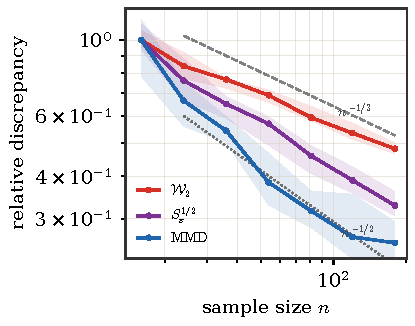
\includegraphics[width=.45\linewidth]{figures/sinkhorn-bias-variance-tradeoff/dimension-3.pdf} &
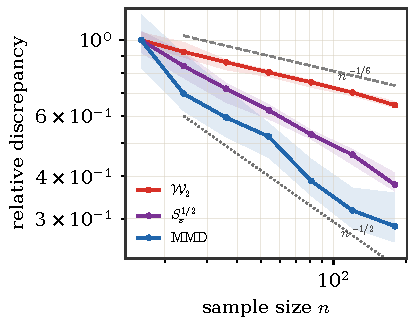
\includegraphics[width=.45\linewidth]{figures/sinkhorn-bias-variance-tradeoff/dimension-6.pdf} \\[-.1em]
\small $d=3$ & \small $d=6$
\end{tabular}
\caption{\emph{Empirical fluctuations in dimensions three and six.} For each sample size $n$, two independent empirical measures $\al_n$ and $\al'_n$ are drawn from the same standard Gaussian law in $\RR^d$. The curves show the median of $\Wass_2$, $\MMD_k$, and $\sqrt{\bar\MK_c^\epsilon}$, each normalized by its first displayed median, with interquartile bands. The Sinkhorn value uses the complete KL-normalized objective, not only the transport term of its regularized plan. Exact OT follows a slower dimension-dependent scale, while MMD and $\sqrt{\bar\MK_c^\epsilon}$ approach the $n^{-1/2}$ guide. For Sinkhorn this guide is the square root of an $n^{-1}$ second-order null statistic, not a first-order fluctuation of the raw divergence.}
\index{Sinkhorn!divergence}% strictindex
\index{empirical!measure}% strictindex
\label{fig:sinkhorn-bias-variance-tradeoff}
\end{figure}

\paragraph{Lower bounds and minimax optimality.}
\index{minimax optimality}% strictindex
\index{minimax lower bound}% strictindex
The empirical upper bound above is not merely a weakness of the plug-in estimator. In fully nonparametric classes, the \(n^{-1/d}\) scale is a genuine minimax obstruction: from \(n\) samples one can resolve only about \(n\) spatial boxes, and the Wasserstein cost of an unresolved signed imbalance is proportional to the box diameter. This idea goes back to Dudley's entropy method and is now understood sharply for empirical measures and minimax distribution estimation in Wasserstein loss~\cite{dudley1969speed,fournier2015rate,singh2018minimax,weed2017sharp,weed2025statistical}. The following elementary application of Assouad's hypercube lemma~\cite{assouad1983deux} gives the basic obstruction already for measures with bounded densities.
\index{minimax lower bound}% strictindex
\index{Assouad lemma}% strictindex
\index{density!estimation}% strictindex

\begin{prop}[Minimax lower bound for bounded densities]\label{prop-minimax-lower-w1-density}
\index{minimax lower bound}% strictindex
\index{Wasserstein!minimax rate}% strictindex
	Let \(d\geq3\). Let \(\mathcal A\) be the class of probability measures on \([0,1]^d\) admitting a density \(\rho\) with respect to Lebesgue measure such that
	$\frac12\leq \rho(x)\leq \frac32$ for a.e.\ $x\in[0,1]^d$.
	For each \(n\geq1\), let \(\mathfrak E_n\) be the class of measurable estimators \(\widetilde\alpha_n:([0,1]^d)^n\to\Pp([0,1]^d)\).
	There exists \(c_d>0\), depending only on \(d\), such that
	\[
		\inf_{\widetilde\alpha_n\in\mathfrak E_n}
		\sup_{\alpha\in\mathcal A}
		\EE_{(X_1,\ldots,X_n)\sim\alpha^{\otimes n}}
		\left[
			\Wass_1\big(\widetilde\alpha_n(X_1,\ldots,X_n),\alpha\big)
		\right]
		\geq
		c_d\,n^{-1/d}.
	\]
	The expectation is over i.i.d.\ samples \(X_i\sim\alpha\). In particular, the high-dimensional rate of Proposition~\ref{prop-empirical-ot-rate} is minimax sharp for \(\Wass_1\), even when one allows arbitrary estimators rather than the empirical measure.
\end{prop}

\begin{proof}
	We use a standard hypercube construction. Choose a smooth function \(\psi\) compactly supported in \((0,1)^d\), with \(\int\psi=0\), \(\norm{\psi}_\infty\leq1\), and whose positive and negative parts are separated in the first coordinate. There exists a compactly supported Lipschitz function \(\varphi\) such that \(\int\varphi\psi\d x>0\). We extend both functions by zero outside \((0,1)^d\), and absorb \(\Lip(\varphi)\) into the constants below.

	Let \(m\) be an integer, \(h=1/m\), and partition \([0,1]^d\) into \(M=m^d\) cubes \(Q_k=z_k+h[0,1)^d\). Define the rescaled bumps
	$\psi_k(x)=\psi\!\left(\frac{x-z_k}{h}\right)\mathbf 1_{Q_k}(x)$.
	For \(\theta=(\theta_1,\ldots,\theta_M)\in\{-1,1\}^M\) and a fixed small \(\eta>0\), set
	$\rho_\theta(x)=1+\eta\sum_{k=1}^M\theta_k\psi_k(x)$ and $\alpha_\theta=\rho_\theta\d x$.
	For \(\eta\) small enough, all these densities belong to \(\mathcal A\), and they integrate to one because every \(\psi_k\) has zero mean.

	If \(\theta\) and \(\theta'\) differ on a set \(S\) of coordinates, the dual formula for \(\Wass_1\) gives an additive lower bound. Indeed, rescale \(\varphi\) as
	\(\varphi_k(x)=h\,\varphi\!\left(\frac{x-z_k}{h}\right)\).
	Each \(\varphi_k\) is supported in a fixed strict subcube of \(Q_k\). Consequently every signed sum \(\sum_k s_k\varphi_k\), \(s_k\in\{-1,0,1\}\), has a Lipschitz constant bounded by a constant depending only on \(\varphi\), uniformly in \(m\) and in the signs. After dividing by this constant, Kantorovich--Rubinstein duality and the choice \(s_k=\operatorname{sign}(\theta_k-\theta'_k)\) on \(S\) give \(\Wass_1(\alpha_\theta,\alpha_{\theta'})\geq c\eta h^{d+1}\mathrm{Ham}(\theta,\theta')\), where \(\mathrm{Ham}\) denotes Hamming distance and \(c>0\) depends only on the chosen bump.

	Neighboring vertices of the hypercube are statistically close. If \(\theta^{[k]}\) is obtained from \(\theta\) by flipping only the \(k\)-th sign, then the one-sample Kullback--Leibler divergence is bounded by
	$\KL(\alpha_\theta|\alpha_{\theta^{[k]}}) \leq C\eta^2 h^d$,
	because the two densities differ only on \(Q_k\), the perturbation has size \(O(\eta)\), and the densities are uniformly bounded away from zero. For \(n\) independent samples the divergence is multiplied by \(n\). Choose \(m\) so that \(m^d\simeq n\). Then \(n h^d\) is bounded, and, by taking \(\eta\) sufficiently small, Pinsker's inequality (Theorem~\ref{thm-pinsker}) gives a uniform bound
	$\TV\big(\alpha_\theta^{\otimes n},\alpha_{\theta^{[k]}}^{\otimes n}\big) \leq q<1$.
	Assouad's lemma~\cite{assouad1983deux} converts this \(M\)-dimensional hypercube into \(M\) binary testing problems. More precisely, if the loss between two vertices is bounded below by \(\delta\) times their Hamming distance, while every pair of one-coordinate neighboring experiments has total variation at most \(q<1\), then every estimator has worst-case expected loss bounded below by a universal constant times \(M\delta(1-q)\). Here \(\delta=c\eta h^{d+1}\), so the lemma gives
	\[
		\inf_{\widetilde\alpha_n\in\mathfrak E_n}
		\sup_{\theta\in\{-1,1\}^M}
		\EE_{\alpha_\theta^{\otimes n}}
		\left[
			\Wass_1\big(\widetilde\alpha_n(X_1,\ldots,X_n),\alpha_\theta\big)
		\right]
		\geq
		c'\eta\,M h^{d+1}(1-q)
		=
		c'\eta(1-q)h
		\simeq
		n^{-1/d}.
	\]
	Decreasing the constant handles the finitely many small values of \(n\), and the claim follows.
\end{proof}

The same packing mechanism gives the corresponding high-dimensional lower bounds for \(\Wass_p\): in the regime \(d>2p\), one obtains the scale \(n^{-1/d}\) for \(\Wass_p\) itself, or \(n^{-p/d}\) for \(\Wass_p^p\); see~\cite{singh2018minimax,weed2017sharp}. For estimating a scalar transport value such as \(\Wass_p(\alpha,\beta)\) at a fixed nondegenerate pair, the minimax picture is more nuanced because the value can be differentiable and have \(n^{-1/2}\) fluctuations, as in Section~\ref{sec-bias-variance-ot}. The lower bound above nevertheless captures the nonparametric obstruction near the diagonal and for distribution recovery: without structural assumptions beyond bounded density or low intrinsic dimension, the curse-of-dimensionality scale cannot be removed by changing the estimator.
\index{plug-in estimator}% strictindex
\index{bias-variance tradeoff}% strictindex

\paragraph{Leveraging smoothness.}
\index{smoothing estimator}% strictindex
\index{smoothed plug-in estimator}% strictindex
\index{Sobolev smoothness}% strictindex
The preceding lower bound concerns rough densities. Sobolev regularity can be exploited by filtering the empirical measure before comparing it with the target. To use smoothness orders beyond one, however, the filter must cancel sufficiently many low-order moments and is therefore generally signed. This is harmless for estimating a \(\Wass_1\) value: the Kantorovich--Rubinstein norm \(\norm{\cdot}_{W_1}\) from~\eqref{eq-w1-metric} is defined on every zero-mass signed measure, and \(\Wass_1(\alpha,\beta)=\norm{\alpha-\beta}_{W_1}\). The following result makes this distinction explicit. At bandwidth \(h\), the bias is of order \(h^{s+1}\), whereas the empirical fluctuation is of order \(n^{-1/2}h^{1-d/2}\). Balancing them gives the smooth-density minimax exponent~\cite{nilesweed2019minimaxSmooth,divol2022measure}.
\index{smoothness}% strictindex
\index{density!estimation}% strictindex
\index{kernel!smoothing}% strictindex

\begin{prop}[Smoothed plug-in rates]\label{prop-smooth-plugin-w1-rate}
\index{smooth density}% strictindex
\index{plug-in estimator}% strictindex
	Let \(d\geq3\), \(s>0\), and let \(\alpha=\density{\alpha}\d x\), \(\beta=\density{\beta}\d x\) be probability measures on the unit-volume flat torus \(\TT^d\), with \(\max\{\norm{\density{\alpha}}_{H^s},\norm{\density{\beta}}_{H^s}\}\leq L\). Choose an even function \(\chi\in\Cc^\infty(\RR^d;[0,1])\) such that \(\chi(\xi)=1\) for \(\norm{\xi}\leq1\) and \(\chi(\xi)=0\) for \(\norm{\xi}\geq2\). For \(0<h\leq1\), let \(\kappa_h\) be the periodic kernel with Fourier coefficients \(\widehat\kappa_h(k)=\chi(hk)\), and define \(\tilde\alpha_{n,h}:=\hat\alpha_n\ast\kappa_h\) and \(\tilde\beta_{m,h}:=\hat\beta_m\ast\kappa_h\). These are signed measures of total mass one. Then
	\[
		\EE\norm{\tilde\alpha_{n,h}-\alpha}_{W_1}
		\leq
		C\left(h^{s+1}+n^{-1/2}h^{1-d/2}\right).
	\]
	The analogous bound holds for \(\tilde\beta_{m,h}-\beta\). Define the signed plug-in estimator
	\[
		\widehat{\Wass}_{1,n,m}
		\eqdef
		\norm{\tilde\alpha_{n,h_n}-\tilde\beta_{m,h_m}}_{W_1}.
	\]
	Choosing \(h_n\simeq n^{-1/(d+2s)}\) and \(h_m\simeq m^{-1/(d+2s)}\) gives
	\[
		\EE\abs{
			\widehat{\Wass}_{1,n,m}
			-
			\Wass_1(\alpha,\beta)}
		\leq
		C\left(n^{-\frac{s+1}{d+2s}}+m^{-\frac{s+1}{d+2s}}\right).
	\]
	The constant depends only on \(d,s,L\) and \(\chi\).
\end{prop}

\begin{proof}
	It suffices to prove the one-sample bound. For a zero-mean function \(w\) on the torus, set
	\[
		\norm{w}_{\dot H^{-1}(\TT^d)}^2
		\eqdef
		\sum_{k\in\ZZ^d\setminus\{0\}}
		\frac{\abs{\widehat w(k)}^2}{4\pi^2\norm{k}^2}.
	\]
	Kantorovich--Rubinstein duality and Cauchy--Schwarz give \(\norm{w\d x}_{W_1}\lesssim\norm{w}_{\dot H^{-1}(\TT^d)}\), because a \(1\)-Lipschitz test function has \(L^2\)-gradient norm at most one on the unit-volume torus. Moreover, \(\EE\tilde\alpha_{n,h}=(\density{\alpha}\ast\kappa_h)\d x\), so the error splits into a deterministic smoothing bias and a centered empirical fluctuation.

	Since \(\chi\) equals one near the origin, for every \(s>0\) one has \(\abs{1-\chi(hk)}\lesssim_s(h\norm{k})^{s+1}\). Fourier estimates and Parseval's identity therefore give
	\[
		\begin{aligned}
			\norm{\density{\alpha}\ast\kappa_h-\density{\alpha}}_{\dot H^{-1}}
			&\lesssim h^{s+1}\norm{\density{\alpha}}_{H^s},\\
			\EE\norm{\density{\tilde\alpha_{n,h}}-\density{\alpha}\ast\kappa_h}_{\dot H^{-1}}^2
			&\lesssim \frac1n\sum_{k\neq0}\frac{\abs{\chi(hk)}^2}{\norm{k}^2}
			\lesssim \frac{h^{2-d}}n.
		\end{aligned}
	\]
	In the second line, the support of \(\chi\) restricts the sum to \(0<\norm{k}\leq2/h\), and \(\sum_{0<\norm{k}\leq2/h}\norm{k}^{-2}\lesssim h^{2-d}\) because \(d\geq3\). The triangle and Jensen inequalities give the one-sample bound. Equating its two terms yields \(h\simeq n^{-1/(d+2s)}\). Finally, the reverse triangle inequality for the norm \(\norm{\cdot}_{W_1}\) gives the two-sample claim.
\end{proof}

\index{smooth OT estimation}% strictindex
\begin{rem}[Kernel order and smoothness adaptation]\label{rem-smooth-plugin-kernel-order}
	Suppose that a unit-mass smoothing kernel has cancellation order \(q>0\), in the sense that
	\[
		\abs{1-\widehat\kappa(\xi)}
		\lesssim
		\min\{1,\norm{\xi}^q\}.
	\]
	The proof above then gives, for \(\rho\in H^s\),
	\[
		\norm{\rho\ast\kappa_h-\rho}_{\dot H^{-1}}
		\lesssim
		h^{\min\{s+1,q\}}\norm{\rho}_{H^s}.
	\]
	Thus the optimal bias \(h^{s+1}\) only requires \(q\geq s+1\). A single Gaussian has \(q=2\), because \(1-e^{-h^2\norm{\xi}^2/2}\sim h^2\norm{\xi}^2/2\), and is therefore sufficient for \(0<s\leq1\). More generally, choose \(r\geq\lceil(s+1)/2\rceil\), distinct scales \(c_1,\ldots,c_r>0\), and coefficients satisfying
	\[
		\sum_{j=1}^r a_j=1
		\qandq
		\sum_{j=1}^r a_jc_j^{2\ell}=0
		\quad (1\leq\ell<r).
	\]
	Then \(\kappa_h=\sum_{j=1}^r a_jG_{c_jh}\), where \(G_h\) is the centered Gaussian density of standard deviation \(h\), has order \(q=2r\). For instance, \(4G_h/3-G_{2h}/3\) has order four and handles every \(0<s\leq3\). Kernels of order greater than two are necessarily signed under the usual nondegeneracy assumptions.

	The flat-top multiplier used in Proposition~\ref{prop-smooth-plugin-w1-rate} has infinite cancellation order and hence works for every \(s>0\): the kernel itself need not be selected from knowledge of \(s\). A kernel suitable for some smoothness is also suitable for every smaller smoothness; only the converse fails. The oracle bandwidth \(h_n\simeq n^{-1/(d+2s)}\), however, does depend on \(s\). Consequently the displayed estimator is not rate-adaptive when \(s\) is unknown. A multiscale bandwidth rule, such as Lepski's method, can be used to seek adaptation, typically at the price of logarithmic factors; this refinement is not developed here. Standard \(\Wass_1\) is not a distance between signed measures, but the Kantorovich--Rubinstein norm used above is well-defined for their zero-mass difference. If a probability-valued estimator is required, one must additionally apply a positivity correction or projection~\cite{nilesweed2019minimaxSmooth,divol2022measure}.
\end{rem}

Dimensions one and two require separate parametric or logarithmic estimates; Proposition~\ref{prop-smooth-plugin-w1-rate} isolates the high-dimensional regime \(d\geq3\). As \(s\) becomes comparable with \(d\), the exponent \((s+1)/(d+2s)\) no longer vanishes with dimension, and it tends to the parametric exponent \(1/2\) as \(s/d\to+\infty\).

Unfortunately, these kernel-smoothed estimators are generally computationally intractable in high dimension: evaluating the resulting continuous Kantorovich--Rubinstein problem requires a spatial discretization whose size grows exponentially with \(d\).
\index{Sobolev space}% strictindex

\paragraph{MMD.}
MMD contains no transport optimization: its square is a combination of expectations of kernel evaluations, estimated empirically by sums of kernel values. Ordinary Monte-Carlo averaging therefore gives the dimension-free parametric rate below for bounded kernels. This sharply contrasts with exact empirical OT, whose value is defined through an optimization problem and whose worst-case \(\Wass_1\) plug-in bias in dimension \(d>2\) decays only as \(n^{-1/d}\), corresponding to a sample requirement of order \(\delta^{-d}\) at accuracy \(\delta\). The constants for MMD still depend on the kernel and its bandwidth, and changing the kernel changes the discrepancy being estimated.
\index{maximum mean discrepancy}% strictindex
\index{kernel!mean embedding}% strictindex
\index{rate!parametric}% strictindex

\begin{prop}[MMD has a parametric value rate]\label{prop-mmd-sample-rate}
\index{maximum mean discrepancy}% strictindex
\index{rate!parametric}% strictindex
	Let $k$ be a bounded positive definite kernel with $k(x,x)\leq\kappa^2$, and let $\MMD_k$ be the discrepancy of Definition~\ref{def-kernel-mmd-norm}. If $\hat\alpha_n$ and $\hat\beta_m$ are independent empirical measures, then
\index{empirical!measure}% strictindex
	\[
		\EE\abs{\MMD_k(\hat\alpha_n,\hat\beta_m)-\MMD_k(\alpha,\beta)}
\index{maximum mean discrepancy}% strictindex
		\leq
		\kappa\left(\frac1{\sqrt n}+\frac1{\sqrt m}\right).
	\]
\end{prop}

\begin{proof}
	Let $\Phi(x)=k(x,\cdot)$ be the feature map and $m_\alpha=\EE\Phi(X)$. The reverse triangle inequality for the RKHS norm gives
\index{triangle inequality}% strictindex
\index{RKHS}% strictindex
	\[
		\abs{\MMD_k(\hat\alpha_n,\hat\beta_m)-\MMD_k(\alpha,\beta)}
\index{maximum mean discrepancy}% strictindex
		\leq
		\MMD_k(\hat\alpha_n,\alpha)+\MMD_k(\hat\beta_m,\beta).
	\]
	Independence cancels the cross terms after taking the squared norm and expectation, giving
	\[
		\EE\MMD_k(\hat\alpha_n,\alpha)^2
		=\frac1n\EE\norm{\Phi(X)-m_\alpha}_{\RKHS_k}^2
		=\frac{1}{n}\Big(\EE k(X,X)-\EE k(X,X')\Big).
	\]
	The same estimate applies to $\hat\beta_m$, and Jensen's inequality together with $k(x,x)\leq\kappa^2$ gives the displayed bound.
\index{Jensen inequality}% strictindex
\end{proof}

\paragraph{Entropic OT.}
Entropic regularization keeps the transport geometry but smooths the dual potentials at scale \(\sqrt\epsilon\). For fixed \(\epsilon>0\), this smoothing reduces empirical fluctuations to a parametric scale, in the same spirit as smooth losses in classical statistics~\cite{genevay2018sample,bigot2017central,mena2019statistical}. The large-\(\epsilon\) limit connects to MMD-type kernel tests~\cite{feydy2018interpolating,gretton2012kernel}; the small-\(\epsilon\) limit recovers exact OT but makes the constants deteriorate. The statistical gain is therefore inseparable from the regularization bias.
\index{entropic!regularization}% strictindex
\index{Sinkhorn!divergence}% strictindex
\index{regularization bias}% strictindex

\begin{prop}[Fixed-temperature Sinkhorn divergence has a parametric rate]\label{prop-sinkhorn-sample-rate}
\index{Sinkhorn!divergence}% strictindex
\index{subgaussian measure}% strictindex
	Let \(c(x,y)=\norm{x-y}^2/2\), and assume that \(\alpha\) and \(\beta\) are \(\sigma^2\)-subgaussian probability measures on \(\RR^d\), in the sense that
	$\int e^{\norm{x}^2/(2d\sigma^2)}\d\alpha(x)\leq2$ and $\int e^{\norm{y}^2/(2d\sigma^2)}\d\beta(y)\leq2$.
	Set
	$q_d\eqdef\left\lceil\frac{5d}{2}\right\rceil+6$ and $\Lambda_{d,\sigma}(\epsilon) \eqdef \epsilon\left[1+\left(\frac{\sigma}{\sqrt\epsilon}\right)^{q_d}\right]$.
	Let \(\hat\alpha_n\) and \(\hat\beta_m\) be independent empirical measures. Then, for every \(\epsilon>0\),
	\[
		\EE\abs{\bar\MK_\c^\epsilon(\hat\alpha_n,\hat\beta_m)-\bar\MK_\c^\epsilon(\alpha,\beta)}
		\leq
		C_d\,\Lambda_{d,\sigma}(\epsilon)
		\left(\frac1{\sqrt n}+\frac1{\sqrt m}\right).
	\]
\end{prop}

\begin{proof}
	Adding a separable term \(a(x)+b(y)\) to the cost adds
	$\int a\d\mu+\int b\d\nu$ to $\MK_c^\epsilon(\mu,\nu)$, because every feasible coupling has marginals $(\mu,\nu)$. When the same function is added on both sides, $b=a$, these marginal terms cancel in the Sinkhorn divergence. Since
	$c(x,y)=\norm{x-y}^2/2=-\dotp{x}{y}+\norm{x}^2/2+\norm{y}^2/2$, we may therefore work throughout the proof with the bilinear cost $c(x,y)=-\dotp{x}{y}$. We first estimate its raw entropic value and then pass to the debiased expression.

	For the measures \(\alpha,\beta\) in the statement, write the dual objective, following~\eqref{eq-dual-sinkhorn-objective}, as
	\[
	\Dd_\epsilon^{\alpha,\beta}(u,v)
	\eqdef
	\int u\d\alpha+\int v\d\beta
	-\epsilon\iint
	\left(
		\exp\left(\frac{u(x)+v(y)-c(x,y)}{\epsilon}\right)-1
	\right)
	\d\alpha(x)\d\beta(y).
	\]
	One can choose normalized optimal potentials for which the Sinkhorn equations hold pointwise on \(\RR^d\)~\cite{mena2019statistical}. Thus, at an optimal pair \((u,v)\),
	$\int \exp\left(\frac{u(x)+v(y)-c(x,y)}{\epsilon}\right) \d\beta(y) =1$ for all $x$.
	Equivalently, the potentials are fixed points of the soft \(c\)-transform, but only the dual normalization is needed below.
	Let \((u,v)\) and \((u_n,v_n)\) be optimal dual potentials for \((\alpha,\beta)\) and \((\hat\alpha_n,\beta)\). By optimality,
	$\Dd_\epsilon^{\alpha,\beta}(u_n,v_n) \leq \Dd_\epsilon^{\alpha,\beta}(u,v)$ and $\Dd_\epsilon^{\hat\alpha_n,\beta}(u,v) \leq \Dd_\epsilon^{\hat\alpha_n,\beta}(u_n,v_n)$.
	Hence the difference of the two optimal values is sandwiched by evaluating the two objectives at these two pairs of potentials. For the pair \((u,v)\) associated with \((\alpha,\beta)\), the preceding Sinkhorn equation cancels the exponential term in the change of the first marginal:
	\[
	\Dd_\epsilon^{\alpha,\beta}(u,v)
	-
	\Dd_\epsilon^{\hat\alpha_n,\beta}(u,v)
	=
	\int u\d(\alpha-\hat\alpha_n).
	\]
	The same identity holds for \((u_n,v_n)\), using its normalization with respect to \(\beta\). Consequently,
	\[
	\abs{\MK_\c^\epsilon(\hat\alpha_n,\beta)-\MK_\c^\epsilon(\alpha,\beta)}
	\leq
	\sup_{w\in\mathcal F_\epsilon(\alpha,\hat\alpha_n;\beta)}
	\abs{\int w\d(\hat\alpha_n-\alpha)},
	\]
	where \(\mathcal F_\epsilon(\alpha,\hat\alpha_n;\beta)\) is the union of the normalized first-marginal potentials for the pairs \((\alpha,\beta)\) and \((\hat\alpha_n,\beta)\). This pathwise class is random; it will be controlled through the subgaussian envelopes below.

	We now set $\epsilon=1$; the general-temperature estimate follows by scaling below. It remains to bound this empirical process uniformly. Set $s_0=\lceil d/2\rceil+1$, and let $\widetilde\sigma_n$ be the smallest common subgaussian proxy for $\alpha$, $\beta$, and $\hat\alpha_n$. This random variable is finite almost surely and satisfies $\EE\widetilde\sigma_n^{2k}\leq C_k\sigma^{2k}$ for every positive integer $k$~\cite{mena2019statistical}. For $\tau\geq0$, let $\mathcal F_{1,\tau}$ denote the class of normalized first-marginal potentials associated with pairs of $\tau^2$-subgaussian measures at unit temperature. The regularity estimates of Mena--Niles-Weed show that every $w\in\mathcal F_{1,\tau}$ satisfies $w/(1+\tau^{3s_0})\in\mathcal F^{s_0}$, where $\mathcal F^{s_0}$ is a fixed polynomial-growth $C^{s_0}$ class whose elements $h$ obey
	\[
		\abs{h(x)}\leq C_{s_0,d}\bigl(1+\norm{x}^2\bigr),
		\qquad
		\abs{D^\kappa h(x)}\leq C_{s_0,d}\bigl(1+\norm{x}^{s_0}\bigr),
		\quad 1\leq|\kappa|\leq s_0.
	\]
	In particular, the preceding random pathwise class is contained in $\mathcal F_{1,\widetilde\sigma_n}$. For a random envelope $L$ controlled by the empirical subgaussian moment, the empirical $L_2$-covering numbers of $\mathcal F^{s_0}$ satisfy
	\[
		\log N(\delta,\mathcal F^{s_0},L_2(\hat\alpha_n))
		\leq
		C_d\,L^{d/(2s_0)}\delta^{-d/s_0}(1+\sigma^{2d}),
	\]
	with $\EE L\leq2$. Since $d/(2s_0)<1$, Dudley's entropy integral is finite. Rademacher symmetrization, the entropy-integral chaining bound~\cite{vanDerVaartWellner1996}, Cauchy--Schwarz, and the moment bounds for $\widetilde\sigma_n$ therefore yield
	\[
	\EE\sup_{w\in\mathcal F_{1,\widetilde\sigma_n}}
	\abs{\int w\d(\hat\alpha_n-\alpha)}
		\leq
		C_d(1+\sigma^{q_d})\,n^{-1/2}.
	\]

	The general \(\epsilon\) case follows by scaling. Set \(\alpha^\epsilon=(D_{1/\sqrt\epsilon})_\sharp\alpha\) and \(\beta^\epsilon=(D_{1/\sqrt\epsilon})_\sharp\beta\). Then
	$\MK_\c^\epsilon(\alpha,\beta) = \epsilon\,\MK_\c^1(\alpha^\epsilon,\beta^\epsilon)$.
	The push-forward of a \(\sigma^2\)-subgaussian law by \(D_{1/\sqrt\epsilon}\) is \((\sigma^2/\epsilon)\)-subgaussian, so the standard-deviation proxy \(\sigma\) is replaced by \(\sigma/\sqrt\epsilon\). The preceding \(\epsilon=1\) estimate therefore gives exactly \(C_d\Lambda_{d,\sigma}(\epsilon)n^{-1/2}\). Keeping this half-integer power avoids an unjustified rounding when $q_d$ is odd and $\epsilon>1$; for $0<\epsilon\leq1$ it can of course be bounded by an integer power of $1/\epsilon$.
	Changing both marginals is handled by the triangle inequality,
	\[
	\abs{\MK_\c^\epsilon(\hat\alpha_n,\hat\beta_m)-\MK_\c^\epsilon(\alpha,\beta)}
	\leq
	\abs{\MK_\c^\epsilon(\hat\alpha_n,\hat\beta_m)-\MK_\c^\epsilon(\alpha,\hat\beta_m)}
	+
	\abs{\MK_\c^\epsilon(\alpha,\hat\beta_m)-\MK_\c^\epsilon(\alpha,\beta)}.
	\]
	The preceding reduction is pathwise: for each realization, it only requires the population and empirical measures appearing in the two terms to share a finite subgaussian proxy. Empirical measures drawn from a subgaussian law have such a random proxy, with moments controlled by the population proxy. Integrating over this proxy gives the two-sample extension~\cite{mena2019statistical}. The argument does not require the two empirical marginals to have the same sample size, so the two contributions scale as \(n^{-1/2}\) and \(m^{-1/2}\).

	Finally, use the definition
	$\bar\MK_\c^\epsilon(\alpha,\beta) = \MK_\c^\epsilon(\alpha,\beta) -\frac12\MK_\c^\epsilon(\alpha,\alpha) -\frac12\MK_\c^\epsilon(\beta,\beta)$.
	The cross term is controlled by the two-marginal estimate. For the self term, use the telescoping inequality
	\[
		\abs{\MK_\c^\epsilon(\hat\alpha_n,\hat\alpha_n)-\MK_\c^\epsilon(\alpha,\alpha)}
		\leq
		\abs{\MK_\c^\epsilon(\hat\alpha_n,\hat\alpha_n)-\MK_\c^\epsilon(\alpha,\hat\alpha_n)}
		+
		\abs{\MK_\c^\epsilon(\alpha,\hat\alpha_n)-\MK_\c^\epsilon(\alpha,\alpha)}.
	\]
	Each term is a one-marginal perturbation in the same pathwise sense: the other marginal may itself be empirical, but it is part of the common random subgaussian class. Thus the self term
	\(\MK_\c^\epsilon(\hat\alpha_n,\hat\alpha_n)-\MK_\c^\epsilon(\alpha,\alpha)\)
	is bounded at the same order as the cross term involving \(\alpha\), and similarly for \(\beta\). Summing these three contributions gives the displayed estimate, up to changing \(C_d\).
\index{Rademacher bound}% strictindex
\index{Dudley entropy}% strictindex
\index{soft!c-transform}% strictindex
\index{empirical!process}% strictindex
\index{dual!potential}% strictindex
\end{proof}

For fixed \(\epsilon>0\), the empirical fluctuation is therefore parametric. Compact support is a special case: if \(\supp(\alpha)\cup\supp(\beta)\subset B(z,R)\), translating both measures by \(-z\) leaves the quadratic transport problem unchanged and the subgaussian assumption holds with \(\sigma=R/\sqrt{2d\log 2}=O(R)\).
Indeed, the integrands in the two subgaussian bounds are then at most \(2\). Genevay--Chizat--Bach--Cuturi--Peyr\'e~\cite{genevay2018sample} established the parametric estimate for compactly supported measures, and Mena--Niles-Weed~\cite{mena2019statistical} extended it to the subgaussian setting above.

\begin{rem}[No free lunch when approximating exact OT]\label{rem-sinkhorn-no-free-lunch}
\index{exact OT}% strictindex
		The parametric rate in Proposition~\ref{prop-sinkhorn-sample-rate} holds for fixed $\epsilon$. If the goal is to approximate the unregularized OT value, one must also account for the regularization bias. A clean $O(\epsilon)$ bound holds when the population supports are fixed and finite. Write $\alpha=\sum_i a_i\delta_{x_i}$, $\beta=\sum_j b_j\delta_{y_j}$, and $\mathsf H(\alpha)=-\sum_i a_i\log a_i$, with the analogous definition for $\beta$. For any coupling $\pi\in\Couplings(\alpha,\beta)$, its relative entropy is the mutual information under $\pi$, and hence
		$\KLD(\pi\mid\alpha\otimes\beta)=I_\pi(X;Y)\leq\min\{\mathsf H(\alpha),\mathsf H(\beta)\}$.
		If the support cardinalities are $N$ and $M$, evaluating the regularized problem at an exact optimal coupling and applying the same estimate to the two self-costs gives
\index{rate!parametric}% strictindex
		\[
			\begin{aligned}
				\abs{\bar\MK_\c^\epsilon(\alpha,\beta)-\MK_\c(\alpha,\beta)}
				&\leq
				\epsilon\left(\log\min\{N,M\}+\frac12\log N+\frac12\log M\right),\\
				\EE\abs{\bar\MK_\c^\epsilon(\hat\alpha_n,\hat\beta_n)-\bar\MK_\c^\epsilon(\alpha,\beta)}
				&\leq C_{d,\sigma}\epsilon^{-p_d}n^{-1/2},
				\qquad p_d\eqdef\frac{q_d}{2}-1.
			\end{aligned}
		\]
		Here the second estimate is the $0<\epsilon\leq1$ form of Proposition~\ref{prop-sinkhorn-sample-rate}, with the factor $\sigma^{q_d}$ absorbed into the constant. Balancing the two terms gives \(\epsilon\simeq n^{-1/(2(p_d+1))}\) and total error of order \(n^{-1/(2(p_d+1))}\) under this conservative fixed-support bound. This calculation is not distribution-free on a continuum: even for compactly supported laws, regularized OT can contain an $\epsilon\log(1/\epsilon)$ term, and cancellation in the Sinkhorn divergence requires additional common-dimensionality and nondegeneracy assumptions~\cite{genevay2018sample,CarlierPegonTamanini2023EntropicRates}. Thus entropic smoothing improves statistical behavior at fixed scale, but approximating exact OT still forces a geometry-dependent bias--variance tradeoff.
\index{exact OT}% strictindex
\index{entropic!smoothing}% strictindex
\end{rem}

\paragraph{Sample complexity of estimating OT maps.}
\index{optimal transport map!estimation}% strictindex
\index{map extrapolation}% strictindex
\index{soft!barycentric projection}% strictindex
\index{optimal transport map!estimation}% strictindex
\index{barycentric!projection}% strictindex
The preceding estimates concern transport values. In many learning tasks, however, one wants the map itself. The standard sample-based principle is to solve the empirical discrete dual problem~\eqref{eq-dual} or its entropic counterpart~\eqref{eq-dual-formulation} for potentials \((\fD_{n,m}^\epsilon,\gD_{n,m}^\epsilon)\in\RR^n\times\RR^m\), where \(\epsilon>0\) denotes the entropic temperature and \(\epsilon=0\) denotes the unregularized Kantorovich problem. The soft \(c\)-transform of Definition~\ref{def-continuous-soft-c-transform} then acts as an extrapolator from the samples to the full ambient space.

For the quadratic cost \(c_2(x,y)=\norm{x-y}^2/2\), let \(X_i\sim\alpha\), \(Y_j\sim\beta\), \(\hat\alpha_n=\sum_i a_i\delta_{X_i}\), \(\hat\beta_m=\sum_j b_j\delta_{Y_j}\), and let \(\P^\epsilon=(\P_{i,j}^\epsilon)\) be the optimal empirical entropic coupling. If \(\gD_{n,m}^\epsilon\) is the target-side dual potential, and if \(\bar c(y,x)\eqdef c_2(x,y)\), define
\[
	u_{n,m}^\epsilon(x)
	\eqdef
	(\gD_{n,m}^\epsilon)^{\bar c,\epsilon}(x)
	=
	-\epsilon\log\sum_j b_j
	\exp\!\left(\frac{\gD_{n,m,j}^\epsilon-c_2(x,Y_j)}{\epsilon}\right),
	\qquad
	T_{n,m}^\epsilon(x)\eqdef x-\nabla u_{n,m}^\epsilon(x).
\]
Equivalently, subtracting the quadratic marginal terms turns \(c_2\) into the bilinear cost \(c_{\rm ip}(x,y)=-\dotp{x}{y}\). With the sign convention used here, the associated soft convex potential is
\[
	\varphi_{n,m}^\epsilon(x)
	\eqdef
	\frac12\norm{x}^2-u_{n,m}^\epsilon(x)
	=
	\epsilon\log\sum_j b_j
	\exp\!\left(
		\frac{\dotp{x}{Y_j}+\gD_{n,m,j}^\epsilon-\frac12\norm{Y_j}^2}{\epsilon}
	\right),
	\qquad
	T_{n,m}^\epsilon=\nabla\varphi_{n,m}^\epsilon.
\]
\index{soft!conjugation}% strictindex
\index{empirical!dual potential}% strictindex
This is the precise form of the informal statement that empirical dual potentials are extended by a soft conjugation and then differentiated. It estimates the Brenier map \(\alpha\to\beta\); the inverse map \(\beta\to\alpha\) is obtained symmetrically from the source-side potential. Differentiating the log-sum-exp gives the explicit half-squared formula
\begin{equation}\label{eq-empirical-entropic-map-barycentric}
	T_{n,m}^\epsilon(x)
	=
	\sum_j \omega_j^\epsilon(x)Y_j,
	\qquad
	\omega_j^\epsilon(x)
	=
	\frac{
		b_j\exp\!\left((\gD_{n,m,j}^\epsilon-c_2(x,Y_j))/\epsilon\right)
	}{
		\sum_k b_k\exp\!\left((\gD_{n,m,k}^\epsilon-c_2(x,Y_k))/\epsilon\right)
	}.
\end{equation}
At a sampled source point \(X_i\), the Sinkhorn normalization gives \(\omega_j^\epsilon(X_i)=\P_{i,j}^\epsilon/a_i\) and \(T_{n,m}^\epsilon(X_i)=a_i^{-1}\sum_j \P_{i,j}^\epsilon Y_j\).
Thus the extrapolated soft-transform map coincides on the empirical support with the barycentric projection~\eqref{eq-barycentric-projection} of the optimal entropic plan. At \(\epsilon=0\), the hard \(c\)-transform is generally nondifferentiable: away from Laguerre boundaries its gradient selects one target site, whereas on a boundary its subdifferential contains several sites. The barycentric projection of an unregularized optimal plan is still well defined on the empirical support, but it need not coincide with a single gradient selection when a row of the plan splits. The following consistency result is therefore stated directly for barycentric projections. It uses uniform empirical weights, as in the usual statistical setting; deterministic nonuniform weights are handled by replacing the grid-entropy estimate in the proof.

\begin{prop}[Consistency of empirical barycentric maps]\label{prop-empirical-barycentric-map-consistency}
\index{optimal transport map!consistency}% strictindex
\index{Brenier!map}% strictindex
	Let \(\Omega\subset\RR^d\) be compact, let \(\alpha,\beta\in\Pp_2(\Omega)\), and assume that \(\alpha\) is absolutely continuous. Let \(\phi\) be a Brenier potential from \(\alpha\) to \(\beta\) for the cost \(c_2(x,y)=\norm{x-y}^2/2\), and choose a bounded Borel selection \(T(x)\in\partial\phi(x)\) on \(\Omega\). At every differentiability point of \(\phi\), this selection necessarily equals \(\nabla\phi(x)\), so it is a representative of the unique Brenier map. Let \(X_i,Y_j\in\Omega\), and assume that \(\hat\alpha_n=n^{-1}\sum_{i=1}^n\delta_{X_i}\to\alpha\) and \(\hat\beta_m=m^{-1}\sum_{j=1}^m\delta_{Y_j}\to\beta\) in \(\Wass_2\). Let \(\epsilon_{n,m}\geq0\) satisfy \(\epsilon_{n,m}\to0\) and \(\epsilon_{n,m}\log(\min\{n,m\})\to0\). For each \(n,m\), let \(\P_{n,m}^{\epsilon}\) be an optimal coupling matrix between \(\hat\alpha_n\) and \(\hat\beta_m\), with \(\epsilon=\epsilon_{n,m}\): unregularized if \(\epsilon=0\), entropic if \(\epsilon>0\). Form the aggregated plan \(\pi_{n,m}^\epsilon=\sum_{i,j}\P_{i,j}^\epsilon\delta_{(X_i,Y_j)}\), disintegrate it as \(\pi_{n,m}^\epsilon(\d x,\d y)=\hat\alpha_n(\d x)\pi_{n,m,x}^\epsilon(\d y)\), and define
	$\bar T_{n,m}^{\epsilon}(x) \eqdef \int y\,\d\pi_{n,m,x}^\epsilon(y)$.
	Equivalently, if \(I_x\eqdef\{i:X_i=x\}\), then
	\[
		\bar T_{n,m}^{\epsilon}(x)
		=
		\frac{n}{|I_x|}\sum_{i\in I_x}\sum_j\P_{i,j}^{\epsilon}Y_j.
	\]
	When the source sites are distinct this reduces to \(\bar T_{n,m}^{\epsilon}(X_i)=n\sum_j\P_{i,j}^{\epsilon}Y_j\). The aggregated definition remains single-valued when sites are repeated and satisfies
	\[
		\int \norm{\bar T_{n,m}^{\epsilon}(x)-T(x)}^2
		\d\hat\alpha_n(x)
		=
		\frac1n\sum_i \norm{\bar T_{n,m}^{\epsilon}(X_i)-T(X_i)}^2
		\longrightarrow0
	\]
	as \(n,m\to+\infty\).
	If \(\beta\) is also absolutely continuous, the analogous backward barycentric projections converge in \(L^2(\hat\beta_m)\) to the Brenier map \(S:\beta\to\alpha\).
\end{prop}

\begin{proof}
	The assumptions imply \(\MK_{c_2}(\hat\alpha_n,\hat\beta_m)\to\MK_{c_2}(\alpha,\beta)\). If \(\epsilon=0\), \(\P_{n,m}^{\epsilon}\) is exactly optimal. If \(\epsilon>0\), compare its entropic objective with an unregularized optimal empirical plan \(Q_{n,m}\). Regarding \(Q_{n,m}\) as the joint law of two uniform discrete indices, its relative entropy with respect to their product law is their mutual information. Hence
	$\KLD(Q_{n,m}|\hat\alpha_n\otimes\hat\beta_m) \leq \min\{\log n,\log m\}$.
		It follows that
		$\int c_2\,\d \pi_{n,m}^{\epsilon} \leq \MK_{c_2}(\hat\alpha_n,\hat\beta_m) +\epsilon\log(\min\{n,m\})$.
		Hence the transport costs of \(\pi_{n,m}^{\epsilon}\) converge to the population optimum. By compactness, every weak limit point of these aggregated plans has marginals \(\alpha,\beta\) and optimal quadratic cost. Brenier uniqueness therefore forces the whole sequence to converge weakly to \((\Id,T)_\sharp\alpha\).

		Disintegrate the aggregated plan \(\pi_{n,m}^{\epsilon}\) with respect to its first marginal and denote its barycentric projection by \(\bar T_{n,m}^{\epsilon}\). Jensen's inequality gives
	\[
		\int \norm{\bar T_{n,m}^{\epsilon}(x)-T(x)}^2\d\hat\alpha_n(x)
		\leq
			\iint \norm{y-T(x)}^2\d \pi_{n,m}^{\epsilon}(x,y).
	\]
	At every differentiability point of \(\phi\), the subdifferential is the singleton \(\{\nabla\phi(x)\}\). Since the target is compact, the relevant subgradients are bounded, and the closed-graph property of \(\partial\phi\) implies continuity of the selected gradient at such a point. Convex functions are differentiable Lebesgue-almost everywhere; because \(\alpha\) is absolutely continuous, the bounded function \((x,y)\mapsto\norm{y-T(x)}^2\) is continuous \((\Id,T)_\sharp\alpha\)-almost everywhere. The portmanteau theorem for bounded functions whose discontinuity set has zero limiting mass gives
	\[
			\iint \norm{y-T(x)}^2\d \pi_{n,m}^{\epsilon}(x,y)
		\longrightarrow
		\iint \norm{y-T(x)}^2\d[(\Id,T)_\sharp\alpha](x,y)=0.
	\]
	The proof for the backward map is identical when the optimal plan is also induced by the Brenier map from \(\beta\) to \(\alpha\).
\index{Jensen inequality}% strictindex
\end{proof}

\index{Brenier!potential stability}% strictindex
\index{entropic!barycentric map}% strictindex
Quantitative map convergence requires stronger regularity than consistency. The following result gives a direct finite-sample guarantee for the Sinkhorn-based estimator~\eqref{eq-empirical-entropic-map-barycentric}~\cite{pooladian2021entropicOTMaps}.

\begin{prop}[Finite-sample rate for the entropic map]\label{prop-entropic-map-rate}
	Assume that \(\alpha\) and \(\beta\) have densities on a common compact set \(\Omega\), both bounded above and with \(\density{\beta}\) bounded below away from zero. Let \(T=\nabla\phi\) be the quadratic Brenier map from \(\alpha\) to \(\beta\), and assume that \(\phi\in C^2(\Omega)\), its Legendre conjugate satisfies \(\phi^*\in C^{s+1}(\Omega)\) for some \(s>1\), and
	\[
		\mu\Id_d\preceq\nabla^2\phi(x)\preceq L\Id_d
		\qquad (x\in\Omega)
	\]
	for constants \(0<\mu\leq L\). Set \(\bar s\eqdef s\wedge3\), assume that \(\mathcal I_{\rm geo}(\alpha,\beta)<+\infty\) as in Proposition~\ref{prop-small-epsilon-expansion}, and draw \(n\) independent samples from each measure. If \(\epsilon_n\simeq n^{-1/(d+\bar s+1)}\), then the estimator \(T_{n,n}^{\epsilon_n}\) defined in~\eqref{eq-empirical-entropic-map-barycentric} satisfies
	\[
		\EE\norm{T_{n,n}^{\epsilon_n}-T}_{L^2(\alpha)}^2
		\lesssim
		\bigl(1+\mathcal I_{\rm geo}(\alpha,\beta)\bigr)
		n^{-\frac{\bar s+1}{2(d+\bar s+1)}}\log n.
	\]
\end{prop}

This estimator is directly computable from Sinkhorn potentials. Under stronger modeling and smoothing assumptions, unregularized estimators can attain sharper minimax rates~\cite{hutter2021minimaxOTMaps,deb2021ratesBarycentricMaps,manole2021pluginOTMaps}.
\index{optimal transport map!estimation}% strictindex
\index{barycentric!projection}% strictindex
\index{entropic!map estimation}% strictindex

\paragraph{Sliced Wasserstein.}
\index{sliced Wasserstein!distance}% strictindex
For a direction \(\theta\in\Sphere^{d-1}\), let \(P_\theta(x)=\dotp{\theta}{x}\) be the one-dimensional projection and let \(\sigma\) denote the normalized surface measure on the sphere. For \(\alpha,\beta\in\Pp_p(\RR^d)\), the sliced Wasserstein distance is
\[
	\SW_p(\alpha,\beta)^p
	\eqdef
	\int_{\Sphere^{d-1}}
	\Wass_p\big((P_\theta)_\sharp\alpha,(P_\theta)_\sharp\beta\big)^p
	\d\sigma(\theta).
\]
This construction keeps genuine one-dimensional transport while avoiding a full high-dimensional matching at every evaluation. It is studied in detail in Section~\ref{sec-sliced-wasserstein}, including its metric properties, Monte-Carlo approximation and variants. Here we record a particularly clean statistical consequence for \(p=1\): empirical fluctuations are controlled through one-dimensional cumulative functions rather than ambient-dimensional matching. This is one of the main motivations for sliced objectives in generative modeling and statistics~\cite{nadjahi2019asymptotic,nadjahi2020statistical,manole2019minimax}.
\index{sliced Wasserstein!distance}% strictindex
\index{sliced Wasserstein!sample complexity}% strictindex
\begin{thm}[Dimension-free empirical rate for \texorpdfstring{$\SW_1$}{sliced Wasserstein-1}]\label{thm-sliced-sample-complexity}
\index{sliced Wasserstein!sample complexity}% strictindex
	Let \(\alpha,\beta\in\Pp(\RR^d)\) satisfy
	\(\supp(\alpha)\cup\supp(\beta)\subset B(0,R)\), and let
	\(\hat\alpha_n\) and \(\hat\beta_m\) be their empirical measures from \(n\) and \(m\) i.i.d.\ samples, respectively. Then
	\[
		\EE\abs{\SW_1(\hat\alpha_n,\hat\beta_m)-\SW_1(\alpha,\beta)}
		\leq
		R\left(\frac{1}{\sqrt n}+\frac{1}{\sqrt m}\right).
	\]
\end{thm}

\begin{proof}
	The triangle inequality for \(\SW_1\) gives
	\[
		\abs{\SW_1(\hat\alpha_n,\hat\beta_m)-\SW_1(\alpha,\beta)}
		\leq
		\SW_1(\hat\alpha_n,\alpha)+\SW_1(\hat\beta_m,\beta).
	\]
	Fix \(\theta\in\Sphere^{d-1}\), set \(\alpha_\theta=(P_\theta)_\sharp\alpha\), and denote the cumulative functions of \(\alpha_\theta\) and its empirical measure by \(F_\theta\) and \(\hat F_{\theta,n}\). Both measures are supported on \([-R,R]\). The one-dimensional identity~\eqref{eq-w1-1d} and the Cauchy--Schwarz inequality give
	\[
		\EE\,\Wass_1\big((P_\theta)_\sharp\hat\alpha_n,\alpha_\theta\big)
		=
		\int_{-R}^R \EE\abs{\hat F_{\theta,n}(s)-F_\theta(s)}\d s
		\leq
		\int_{-R}^R \sqrt{\frac{F_\theta(s)(1-F_\theta(s))}{n}}\d s
		\leq
		\frac{R}{\sqrt n}.
	\]
	Indeed, \(n\hat F_{\theta,n}(s)\) is binomial with success probability \(F_\theta(s)\). Integrating this bound over \(\theta\) yields \(\EE\,\SW_1(\hat\alpha_n,\alpha)\leq R/\sqrt n\). The same argument for \(\beta\), followed by the preceding triangle inequality, proves the result.
\end{proof}

\begin{rem}[Directions are another sample budget]\label{rem-sliced-direction-sample-budget}
\index{sliced Wasserstein!Monte Carlo directions}% strictindex
	The theorem concerns the statistical samples used to form \(\hat\alpha_n\) and \(\hat\beta_m\). In computation, draw i.i.d.\ directions \(\theta_1,\ldots,\theta_L\) with law \(\sigma\), independently of the data, and use the random estimator
	\begin{equation}\label{eq-empirical-direction-sliced-w1}
		\widehat{\SW}_1^{\,L}(\hat\alpha_n,\hat\beta_m)
		\eqdef
		\frac1L\sum_{r=1}^L
		\Wass_1\big((P_{\theta_r})_\sharp\hat\alpha_n,
		(P_{\theta_r})_\sharp\hat\beta_m\big).
	\end{equation}
	Conditionally on the samples, the summands are i.i.d., take values in \([0,2R]\), and have mean \(\SW_1(\hat\alpha_n,\hat\beta_m)\). Their conditional variance is at most \(R^2\), so their mean absolute Monte-Carlo error is at most \(R/\sqrt L\). Combining this estimate with Theorem~\ref{thm-sliced-sample-complexity} gives the joint bound
	\begin{equation}\label{eq-sliced-joint-sample-direction-rate}
		\EE\abs{
		\widehat{\SW}_1^{\,L}(\hat\alpha_n,\hat\beta_m)
		-\SW_1(\alpha,\beta)}
		\leq
		R\left(\frac1{\sqrt L}+\frac1{\sqrt n}+\frac1{\sqrt m}\right).
	\end{equation}
	Thus the directional approximation preserves the empirical rate provided
	\(L\gtrsim\min\{n,m\}\); more precisely, its contribution is no larger than the two-sample contribution whenever
	\(L\geq(n^{-1/2}+m^{-1/2})^{-2}\).
	If only \(\alpha\) is sampled while \(\beta\) is known, the corresponding bound is
	\(R(L^{-1/2}+n^{-1/2})\), and retaining the \(n^{-1/2}\) rate requires \(L\gtrsim n\).
\end{rem}

%%%%%%%%%%%%%%%%%%%%%%%%%%%%%%%%%%%%%%%%%%%%%%%%%%%%%%%%%%%%%%%%%%%%%%%%%%%
\section{Bias and Variance of OT}
\label{sec-bias-variance-ot}
\index{bias}% strictindex
\index{variance}% strictindex
\index{central limit theorem!optimal transport}% strictindex

\paragraph{Bias, variance and approximation errors.}
The previous section answered a coarse but essential question: how many samples are needed before an empirical OT quantity is accurate, typically up to universal constants. We now ask for a finer statistical description of the KL-normalized entropic OT value \(\MK_c^\epsilon\) from Definition~\ref{def-continuous-entropic-ot}, with the convention
\(\MK_c^0\eqdef\MK_c\) for unregularized OT\@. Fixing \(c\), \(\alpha\) and \(\beta\), define the statistical bias
\[
	B_{n,m}^\epsilon
	\eqdef
	\EE \MK_c^\epsilon(\hat\alpha_n,\hat\beta_m)
	-\MK_c^\epsilon(\alpha,\beta)
\]
and the centered fluctuation
\[
	Z_{n,m}^\epsilon
	\eqdef
	\MK_c^\epsilon(\hat\alpha_n,\hat\beta_m)
	-\EE \MK_c^\epsilon(\hat\alpha_n,\hat\beta_m).
\]
If the target is the exact cost but the statistic is entropically regularized, these quantities isolate the three sources of error:
\[
	\MK_c^\epsilon(\hat\alpha_n,\hat\beta_m)-\MK_c^0(\alpha,\beta)
	=
	\underbrace{\MK_c^\epsilon(\alpha,\beta)-\MK_c^0(\alpha,\beta)}_{\text{regularization bias}}
	+
	\underbrace{B_{n,m}^\epsilon}_{\text{statistical bias}}
	+
	\underbrace{Z_{n,m}^\epsilon}_{\text{centered fluctuation}}.
\]
For the debiased Sinkhorn divergence, define \(\bar B_{n,m}^\epsilon\) and \(\bar Z_{n,m}^\epsilon\) by replacing \(\MK_c^\epsilon\) with \(\bar\MK_c^\epsilon\) above; the same decomposition then holds with bars. It is usually read after choosing a temperature \(\epsilon=\epsilon_n\). At fixed \(\epsilon>0\) and on finite supports, the statistical bias is typically \(O(n^{-1}+m^{-1})\), while the centered fluctuation is \(O_\PP(n^{-1/2}+m^{-1/2})\). At fixed temperature the regularization bias does not vanish in general; sending \(\epsilon\to0\) controls it uniformly in standard approximation regimes, although degenerate problems with a uniquely forced product coupling can already have zero bias. The fluctuation constants can deteriorate as \(\epsilon\to0\). This is the bias--variance tradeoff illustrated in Figure~\ref{fig:sinkhorn-bias-variance-tradeoff}.
\index{regularization bias}% strictindex
\index{statistical bias}% strictindex
\index{centered fluctuation}% strictindex

The remainder of this section analyzes the latter two terms. The superscript records their dependence on the regularization strength. The multivariate central limit theorem describes the linear fluctuations of \(\sqrt n(\hat\alpha_n-\alpha)\) against finitely many test functions. Here that empirical process is pushed through the nonlinear transport value \(\MK_c^\epsilon\), which can be nonsmooth at \(\epsilon=0\). The resulting law is governed by its local differentiability and by the geometry of its optimal dual potentials.
\index{empirical!process}% strictindex
\index{dual!potential}% strictindex
\index{entropic!OT}% strictindex

For exact OT on finite spaces, empirical central-limit theorems follow from a directional delta method~\cite{sommerfeld2018inference,tameling2017empirical}; fixed positive entropic regularization makes the transport value smooth on the interiors of the marginal simplices~\cite{bigot2017central,klatt2020empirical,hundrieser2021limit,mena2019statistical}. The following statement isolates the Gaussian regime common to both settings: at zero temperature, uniqueness of the dual potentials turns the directional derivative into an ordinary linear derivative.
\index{finite space}% strictindex
\index{delta method}% strictindex
\index{entropic!regularization}% strictindex

\begin{prop}[Finite-space bias and CLT for OT]\label{prop-finite-ot-clt}
\index{central limit theorem!optimal transport}% strictindex
	Let \(\alpha=\sum_{i=1}^{N}a_i\delta_{x_i}\) and \(\beta=\sum_{j=1}^{M}b_j\delta_{y_j}\), where all weights are positive and \(c\) is finite on the product support. Let \(\hat\alpha_n\) and \(\hat\beta_n\) be the independent empirical laws of \(n\) i.i.d.\ samples from \(\alpha\) and \(\beta\), respectively. Fix \(\epsilon\geq0\), with \(\MK_c^0=\MK_c\), and let \((f_\epsilon^\star,g_\epsilon^\star)\) be optimal dual potentials for \(\MK_c^\epsilon(\alpha,\beta)\). When \(\epsilon=0\), assume that this pair is unique up to the additive gauge; for \(\epsilon>0\), this uniqueness follows after fixing the gauge. Define
	\[
		\mathsf{v}_\epsilon
		\eqdef
		\sum_{i=1}^{N}a_i\bigl(f_\epsilon^\star(x_i)-\bar f_\epsilon\bigr)^2
		+
		\sum_{j=1}^{M}b_j\bigl(g_\epsilon^\star(y_j)-\bar g_\epsilon\bigr)^2,
	\]
	where \(\bar f_\epsilon=\sum_i a_i f_\epsilon^\star(x_i)\) and \(\bar g_\epsilon=\sum_j b_j g_\epsilon^\star(y_j)\). Then, as \(n\to+\infty\) with \(N,M\) fixed,
	\[
		\sqrt n\,B_{n,n}^\epsilon\longrightarrow0,
		\qquad
		\sqrt n\,Z_{n,n}^\epsilon\overset{\mathrm{law}}{\longrightarrow}\Gaussian(0,\mathsf{v}_\epsilon),
		\qquad
		n\,\operatorname{Var}\!\left[\MK_c^\epsilon(\hat\alpha_n,\hat\beta_n)\right]
		\longrightarrow\mathsf{v}_\epsilon.
	\]
	Equivalently,
	\[
		\sqrt n\left(
		\MK_c^\epsilon(\hat\alpha_n,\hat\beta_n)
		-
		\MK_c^\epsilon(\alpha,\beta)
		\right)
		\overset{\mathrm{law}}{\longrightarrow}\Gaussian(0,\mathsf{v}_\epsilon).
	\]
	For every fixed \(\epsilon>0\), one moreover has \(B_{n,n}^\epsilon=O(n^{-1})\).
\end{prop}

\begin{proof}
	Writing \(\hat\a_n\) and \(\hat\b_n\) for the two empirical histograms, the independent multinomial central-limit theorems give \(\sqrt n(\hat\a_n-\a,\hat\b_n-\b)\overset{\mathrm{law}}{\longrightarrow}(G_\a,G_\b)\), where \(G_\a\) and \(G_\b\) are independent centered Gaussian vectors with covariance matrices \(\diag(\a)-\a\a^\top\) and \(\diag(\b)-\b\b^\top\). Proposition~\ref{prop-ot-first-variations-unregularized} gives the directional derivative for every \(\epsilon\geq0\); it is linear under the assumed uniqueness at \(\epsilon=0\), and automatically at positive temperature. Thus,
	\[
		D\MK_c^\epsilon(\alpha,\beta)[h,k]
		=
		\sum_i f_\epsilon^\star(x_i)h_i
		+
		\sum_j g_\epsilon^\star(y_j)k_j.
	\]
	The finite-dimensional delta method~\cite{vanDerVaartWellner1996} therefore gives the centered Gaussian limit stated in the proposition. Independence and the two multinomial covariance formulas give its variance \(\mathsf{v}_\epsilon\).

	It remains to justify convergence of the moments, which does not follow from convergence in distribution alone. Set \(R\eqdef\max_{i,j}c(x_i,y_j)-\min_{i,j}c(x_i,y_j)\). Exact dual potentials may be replaced by their \(c\)-transforms, and entropic potentials by their soft \(c\)-transforms; in either case their oscillations are at most \(R\). Since differences of histograms have zero sum, integrating the corresponding subgradient bounds along segments in the two marginal simplices gives \(\abs{\MK_c^\epsilon(\alpha',\beta')-\MK_c^\epsilon(\alpha,\beta)}\leq\frac{R}{2}(\norm{\a'-\a}_1+\norm{\b'-\b}_1)\) for any histograms \((\a',\b')\) and their associated measures \((\alpha',\beta')\). Because \(N,M\) are fixed, the fourth moments of \(\sqrt n\norm{\hat\a_n-\a}_1\) and \(\sqrt n\norm{\hat\b_n-\b}_1\) are uniformly bounded. The squared rescaled OT values are therefore uniformly integrable. The Gaussian limit then yields convergence of the means and second moments, which proves the assertions for \(B_{n,n}^\epsilon\), \(Z_{n,n}^\epsilon\), and the variance.

	For fixed \(\epsilon>0\), the entropic value is twice continuously differentiable in a neighborhood of the positive pair \((\a,\b)\). On that neighborhood, a second-order Taylor expansion has a uniformly bounded remainder; its linear term has zero expectation and \(\EE(\norm{\hat\a_n-\a}^2+\norm{\hat\b_n-\b}^2)=O(n^{-1})\). The probability of leaving the neighborhood is exponentially small, and the preceding global Lipschitz bound controls its contribution. Hence \(B_{n,n}^\epsilon=O(n^{-1})\).
\index{multinomial distribution}% strictindex
\index{delta method}% strictindex
\end{proof}

The uniqueness assumption at \(\epsilon=0\) is substantive. Without it, the directional delta method generally gives a non-Gaussian limit. Its expectation need not vanish, so the exact-OT bias can then have order \(n^{-1/2}\), rather than being negligible at the central-limit scale~\cite{sommerfeld2018inference,tameling2017empirical}.

\paragraph{Fixed support versus a continuum.}
Proposition~\ref{prop-finite-ot-clt} keeps the support sizes \(N\) and \(M\) fixed while \(n\) grows. More explicitly, its limiting variable is
\[
	\sum_{i=1}^{N}f_\epsilon^\star(x_i)(G_\a)_i
	+
	\sum_{j=1}^{M}g_\epsilon^\star(y_j)(G_\b)_j,
	\qquad
	\begin{cases}
	\operatorname{Cov}(G_\a)=\diag(\a)-\a\a^\top,\\
	\operatorname{Cov}(G_\b)=\diag(\b)-\b\b^\top.
	\end{cases}
\]
The variance does not necessarily diverge with \(N,M\): for a uniformly bounded cost, normalized dual potentials have bounded oscillation, hence \(\mathsf{v}_\epsilon\) remains bounded. What fails to be uniform is the differentiability argument. If \(a_{\min}=\min_i a_i\) and \(b_{\min}=\min_j b_j\), then
\[
	\PP[\text{some source or target atom is unobserved}]
	\leq
	N e^{-n a_{\min}}+M e^{-n b_{\min}}.
\]
For uniform weights, the source contribution is at most $\delta/2$ as soon as $n\geq N[\log N+\log(2/\delta)]$, and the analogous target condition uses $M$. Thus a vanishing failure probability requires $n/N-\log N\to+\infty$ and $n/M-\log M\to+\infty$; nearly uniform weights have the same scale up to constants. Moreover, exact-dual uniqueness margins can close as the supports become dense, while entropic Hessian bounds can deteriorate with the smallest weights and as \(\epsilon\downarrow0\). Thus the constant hidden in the bias estimate may grow even when the first-order variance stays bounded.

There is therefore no distribution-free passage from this multinomial CLT to arbitrary continuous laws. Continuous CLTs nevertheless hold under hypotheses ensuring stable unique potentials, with limiting variance \(\operatorname{Var}_\alpha(f_\epsilon^\star)+\operatorname{Var}_\beta(g_\epsilon^\star)\) in the independent two-sample setting~\cite{delBarrioLoubes2017clt,delBarrioGonzalezSanzLoubes2021central,mena2019statistical,gonzalezSanzHundrieser2023weak}. At the diagonal, exact OT has no universal vanishing first derivative. For example, on $\{0,1\}$ with unit ground distance, set
\[
	\alpha_t=\left(\frac{1+t}{2},\frac{1-t}{2}\right),
	\qquad
	\beta_t=\left(\frac{1-t}{2},\frac{1+t}{2}\right).
\]
Then $\Wass_p(\alpha_t,\beta_t)^p=t$ and $\Wass_p(\alpha_t,\beta_t)=t^{1/p}$. Thus the right directional derivative of $\Wass_p^p$ at $t=0$ is nonzero, while that of $\Wass_p$ is nonzero for $p=1$ and infinite for $p>1$. Finite or disconnected supports and empirical perturbations can therefore remain first order and have non-Gaussian limits~\cite{sommerfeld2018inference}. In a smooth connected model, by contrast, regular mass-preserving perturbations have a norm-like first-order expansion for $\Wass_p$; only $\Wass_p^p$ with $p>1$ then has vanishing first variation. The empirical null cost is nevertheless governed by the dimension-dependent matching behavior of Section~\ref{sec-sample-complexity}. For fixed $\epsilon>0$, the first variation of the debiased Sinkhorn divergence cancels under the differentiability assumptions of the second-order delta method, yielding an $n$-scaled quadratic-form limit that may be degenerate~\cite{goldfeld2022limit}.
\index{curse of dimensionality}% strictindex
\index{Sinkhorn!divergence}% strictindex
\index{second-order limit}% strictindex

%%%%%%%%%%%%%%%%%%%%%%%%%%%%%%%%%%%%%%%%%%%%%%%%%%%%%%%%%%%%%%%%%%%%%%%%%%%

\section{Sketching Sinkhorn in Linear Time}
\index{Sinkhorn!linear-time}% strictindex
\index{kernel!sketching}% strictindex
\index{feature sketch}% strictindex
\label{sec-sketching-sinkhorn}
\index{Sinkhorn!sketching}% strictindex
\index{Sinkhorn!linear-time}% strictindex
\index{positive!random features}% strictindex
\index{kernel!low-rank approximation}% strictindex
\index{kernel!sample complexity}% strictindex

The statistical results above explain why entropic OT is attractive at fixed temperature, but they also expose a computational tension. Sampling the marginals replaces the input laws by empirical measures and reduces the problem to finitely many support points; subsampling or coarsening these supports is governed by the sample-complexity estimates of this chapter. Even after the supports are fixed, however, a Sinkhorn sweep costs \(O(nm)\), because it repeatedly applies the Gibbs kernel to vectors. Kernel sketching attacks this second bottleneck: it keeps the sampled marginals fixed and samples, or otherwise compresses, the feature representation of the kernel used by Sinkhorn. With a rank \(R\) factorization, \(N_{\rm it}\) scaling sweeps cost \(O(N_{\rm it}(n+m)R)\), which is linear in the support sizes only when the required rank and iteration count are controlled. The approximation rank generally depends on the ambient or intrinsic dimension, the temperature, and the target accuracy.

\paragraph{PSD kernels and ordinary feature sketches.}
\index{positive!semidefinite kernel}% strictindex
\index{random features}% strictindex
\index{Fourier features}% strictindex
The RKHS/MMD section, Section~\ref{sec-rkhs-mmd}, already used positive semidefinite kernels to define Hilbertian discrepancies between measures. Recall that a symmetric kernel \(k:\Xx\times\Xx\to\RR\) is positive semidefinite if, for every finite family \((x_i)_{i=1}^n\), the Gram matrix \((k(x_i,x_j))_{i,j}\) is positive semidefinite. Many scalable kernel methods start from an integral feature representation
\[
	k(x,y)=\int_Z \dotp{\phi(x,z)}{\phi(y,z)}_{\RR^p}\,d\xi(z),
	\qquad
	\phi:\Xx\times Z\to\RR^p,
\]
where \(\xi\) is a latent probability measure. Drawing \(z_1,\ldots,z_r\sim\xi\) gives the Monte-Carlo sketch
\[
	\widetilde k_r(x,y)
	=
	\frac1r\sum_{\ell=1}^r
	\dotp{\phi(x,z_\ell)}{\phi(y,z_\ell)}_{\RR^p}.
\]
This is the classical random-feature principle. Given two point families \((x_i)_{i=1}^n\) and \((y_j)_{j=1}^m\), define the rectangular cross-kernel matrix \(K\in\RR^{n\times m}\) by \(K_{i,j}=k(x_i,y_j)\). Set \(R=rp\), flatten \((\ell,q)\) into a single feature index, and define
\eql{\label{eq-rectangular-feature-sketch}
	(\Phi_X)_{i,(\ell,q)}=r^{-1/2}\phi_q(x_i,z_\ell),
	\qquad
	(\Phi_Y)_{j,(\ell,q)}=r^{-1/2}\phi_q(y_j,z_\ell),
	\qquad
	\widetilde K=\Phi_X\Phi_Y^\top.
}
Here \(\Phi_X\in\RR^{n\times R}\), \(\Phi_Y\in\RR^{m\times R}\), and
\[
	\widetilde K_{i,j}
	=
	\frac1r\sum_{\ell=1}^r
	\dotp{\phi(x_i,z_\ell)}{\phi(y_j,z_\ell)}_{\RR^p}
	=
	\widetilde k_r(x_i,y_j).
\]
Although \(K\) is generally rectangular and hence is not itself a Gram matrix, it is a cross-block of the Gram matrix evaluated on the union of the two point families. When the families coincide, \(\Phi_X=\Phi_Y=\Phi\), and the construction reduces to the symmetric approximation \(\widetilde K=\Phi\Phi^\top\). The number \(r\) of sampled latent variables is thus a second sample size, distinct from \(n\) and \(m\). At this stage no positivity of \(\phi\) is assumed; signed or oscillatory features are exactly what make Fourier sketches useful.
\index{positive!semidefinite kernel}% strictindex
\index{random features}% strictindex
\index{kernel!ridge regression}% strictindex

For translation-invariant kernels on \(\RR^d\), Bochner's theorem gives the standard Fourier sketch. If \(k(x,y)=\kappa(x-y)\) and \(\kappa(t)=\int e^{\mathrm{i}\dotp{\omega}{t}}\,d\Lambda(\omega)\), then \(\Lambda(\RR^d)=\kappa(0)\). For $\kappa(0)>0$, sample $\omega$ from the probability measure $\rho=\Lambda/\kappa(0)$ and use the real feature
$\phi(x,\omega)=\sqrt{\kappa(0)}(\cos\dotp{\omega}{x},\sin\dotp{\omega}{x})$.
For the normalized Gaussian kernel \(k_\sigma(x,y)=\exp(-\norm{x-y}^2/(2\sigma^2))\), one has $\kappa(0)=1$ and \(\omega\sim\Gaussian(0,\sigma^{-2}\Id)\). This random Fourier feature construction was introduced by Rahimi and Recht to accelerate large-scale kernel machines~\cite{RahimiRecht2007RandomFeatures}; its statistical role for kernel ridge regression and related supervised methods is analyzed, for instance, in~\cite{RudiRosasco2017RandomFeatures,AvronKapralovMusco2017RandomFourierKRR}.
\index{Fourier random features}% strictindex
\index{Bochner theorem}% strictindex
\index{Gaussian!kernel}% strictindex

The following concentration bound assesses the entrywise quality of the rectangular sketch~\eqref{eq-rectangular-feature-sketch}. This is the relevant control when the kernel will subsequently be used inside logarithms or componentwise divisions. A bound on $k(x,y)$ alone controls only the mean of each random feature product, so concentration requires a bound on the feature products themselves.

\begin{prop}[Entrywise accuracy of rectangular feature sketches]
\label{prop-sinkhorn-sketch-positive-guarantee}
\index{kernel!logarithmic accuracy}% strictindex
\index{kernel!positivity}% strictindex
Let \(z_1,\ldots,z_r\) be independent with law \(\xi\), and let \(K_{i,j}=k(x_i,y_j)\) and \(\widetilde K\) be the rectangular kernel matrix and sketch defined above, with \(\widetilde K\) given by~\eqref{eq-rectangular-feature-sketch}. Assume that, for some \(M<+\infty\),
$\abs{\dotp{\phi(x,z)}{\phi(y,z)}_{\RR^p}}\leq M$ for all $x,y$ and $\xi$-a.e.\ $z$.
If \(K_{\min}\eqdef\min_{i,j}K_{i,j}>0\), then, for every \(0<\delta\leq1/2\),
\eql{\label{eq-rectangular-sketch-relative-concentration}
	\PP\pa{
		\max_{i,j}\abs{\frac{\widetilde K_{i,j}}{K_{i,j}}-1}>\delta
	}
	\leq
	2nm\exp\pa{-\frac{rK_{\min}^2\delta^2}{2M^2}}.
}
On the complementary event, \(\widetilde K\) is entrywise positive and, for every \(\epsilon>0\),
\[
	\max_{i,j}
	\abs{-\epsilon\log\widetilde K_{i,j}+\epsilon\log K_{i,j}}
	\leq 2\epsilon\delta.
\]
\end{prop}

\begin{proof}
For each fixed \((i,j)\), the summands in the definition of \(\widetilde K_{i,j}\) have expectation \(K_{i,j}\) and lie in \([-M,M]\). Hoeffding's inequality therefore gives
\[
	\PP\pa{
		\abs{\widetilde K_{i,j}-K_{i,j}}>\delta K_{i,j}
	}
	\leq
	2\exp\pa{-\frac{r\delta^2K_{i,j}^2}{2M^2}}
	\leq
	2\exp\pa{-\frac{r\delta^2K_{\min}^2}{2M^2}}.
\]
A union bound over the \(nm\) entries proves~\eqref{eq-rectangular-sketch-relative-concentration}. On its complementary event, write \(\widetilde K_{i,j}=K_{i,j}(1+s_{i,j})\), where \(\abs{s_{i,j}}\leq\delta\leq1/2\). Hence \(\widetilde K_{i,j}>0\), and \(\abs{\log(1+s_{i,j})}\leq2\abs{s_{i,j}}\) gives the logarithmic estimate.
\end{proof}

\paragraph{Application to Sinkhorn kernels.}
\index{Sinkhorn!kernel}% strictindex
Let $\alpha=\sum_{i=1}^n a_i\delta_{x_i}$ and $\beta=\sum_{j=1}^m b_j\delta_{y_j}$, and write $\a=(a_i)_i$ and $\b=(b_j)_j$ for their weight vectors.
Specialize the preceding construction to the Gibbs kernel \(k_\epsilon(x,y)=e^{-c(x,y)/\epsilon}\), assumed to be PSD and to admit the displayed feature representation. Thus the rectangular matrix defined above is precisely the Sinkhorn kernel, \(K_{i,j}=k_\epsilon(x_i,y_j)\). Assume that the weights and the entries of \(K\) are positive. Recall the Sinkhorn scaling equations~\eqref{eq-sinkhorn}:
$u=\frac{\a}{Kv}$ and $v=\frac{\b}{K^\top u}$,
where divisions are componentwise. Replacing \(K\) by its rank-\(R\) sketch~\eqref{eq-rectangular-feature-sketch}, the two matrix-vector products are evaluated as
\[
	\widetilde K v=\Phi_X(\Phi_Y^\top v),
	\qquad
	\widetilde K^\top u=\Phi_Y(\Phi_X^\top u),
\]
so each scaling sweep costs \(O((n+m)R)\) operations and stores only \(O((n+m)R)\) numbers. The difficulty is that Sinkhorn is not a generic kernel method: it divides by \(\widetilde K v\) and, in dual variables, applies logarithms. Thus one needs \(\widetilde K_{i,j}>0\), preferably with a relative error on the entries, because \(-\epsilon\log K_{i,j}\) is the effective cost. This is a more stringent requirement than the usual spectral or Frobenius approximation of a PSD Gram matrix.
\index{Gibbs!kernel}% strictindex
\index{matrix-vector product}% strictindex

\index{kernel!positivity}% strictindex
\index{logarithmic kernel approximation}% strictindex
\index{Hoeffding inequality}% strictindex
\index{relative!error}% strictindex
\index{logarithmic error}% strictindex
\index{effective rank}% strictindex
\index{Sinkhorn!near-linear}% strictindex
The interaction between kernel accuracy and scaling accuracy can be quantified for Gaussian kernels. The theorem of Altschuler, Bach, Rudi and Niles-Weed~\cite{AltschulerBachRudiWeed2018QuadraticTransport,AltschulerBachRudiNilesWeed2019NystromSinkhorn} is stated for two histograms on a common support, so we retain that setting here rather than implicitly extending it to a rectangular source--target block. We use \(\epsilon\) for the entropic temperature and \(\tau\) for the requested numerical accuracy, and write \(\widetilde O\) for bounds up to logarithmic factors in \(N\), \(1/\tau\), and \(1/\delta\).

Given common-support points \(z_1,\ldots,z_N\in B(0,D)\), an entropic temperature \(\epsilon\), and a target accuracy \(\tau\), form the Gaussian matrix \(K_{i,j}=e^{-\norm{z_i-z_j}^2/\epsilon}\). The Nystr\"om--Sinkhorn method first sets
\[
	\zeta\eqdef\min\left\{1,
		\frac{\tau/\epsilon}{50\bigl(4D^2/\epsilon+\log(N\epsilon/\tau)\bigr)}\right\},
	\qquad
	\rho\eqdef\frac{\zeta}{2}e^{-4D^2/\epsilon}.
\]
Its adaptive randomized column sampler doubles the number of sampled landmarks until its stopping rule for tolerance \(\rho\) is met. If \(I\subset\{1,\ldots,N\}\) is the resulting landmark set, it forms \(V=K_{:,I}\), \(A=K_{I,I}\), and stores only the rank-at-most-\(R\) factorization
\[
	\widetilde K=VA^\dagger V^\top,
	\qquad R=\abs{I},
\]
where \(A^\dagger\) is the Moore--Penrose inverse. Approximate Sinkhorn scaling of \(\widetilde K\) to tolerance \(\zeta\) yields diagonal factors \(D_1,D_2\) and an objective estimate \(\widehat W\); a final marginal-rounding step transforms \(D_1\widetilde K D_2\) into a feasible coupling \(\widehat{\P}\). Neither \(\widetilde K\) nor \(\widehat{\P}\) is formed densely: all scaling and rounding operations use products with \(V\) and \(A^\dagger\). The following proposition certifies this procedure.

\begin{prop}[Accuracy and complexity of Gaussian Nystr\"om--Sinkhorn]
\label{prop-gaussian-nystrom-sinkhorn-complexity}
Let \(z_1,\ldots,z_N\in B(0,D)\subset\RR^d\), where \(N\geq2\) and \(D>1\), and let \(\alpha=\sum_{i=1}^N a_i\delta_{z_i}\) and \(\beta=\sum_{i=1}^N b_i\delta_{z_i}\) have positive weights. Write \(\a=(a_i)_i\), \(\b=(b_i)_i\), and \(\C_{i,j}=\norm{z_i-z_j}^2\). Fix \(\epsilon\in[1/N,1]\) and \(\tau,\delta\in(0,1)\), and apply the preceding Nystr\"om--Sinkhorn procedure. Its kernel approximation \(\widetilde K\) is entrywise positive, and it returns a feasible coupling \(\widehat{\P}\in\CouplingsD(\a,\b)\) and a value \(\widehat W\) satisfying
\[
	0\leq
		\dotp{\C}{\widehat{\P}}
		+\epsilon\KL(\widehat{\P}\,|\,\a\otimes\b)
	-\MK_c^\epsilon(\alpha,\beta)
	\leq\tau,
	\qquad
	\abs{\widehat W-\MK_c^\epsilon(\alpha,\beta)}\leq\tau.
\]
With probability at least \(1-\delta\), the selected sketch rank satisfies
\eql{\label{eq-gaussian-nystrom-rank}
	R
	\lesssim_d
	\pa{
		1+\frac{D^2}{\epsilon}
		+\log\frac{N(1+D^2)}{\tau}
	}^d
	\log\frac{N}{\delta},
}
and the complete computation uses
\[
	\widetilde O\pa{
		NR\pa{R+\frac{D^4}{\epsilon\tau}}
	}
	\quad\text{operations and}\quad
	O\pa{N(R+d)}
	\quad\text{memory}.
\]
Here the constant hidden in \(\lesssim_d\) depends only on \(d\).
\end{prop}

\begin{proof}
Set the inverse temperature \(\eta=1/\epsilon\). The assumptions above are precisely the normalized range \(\eta\in[1,N]\), \(D>1\), and \(\tau\leq1\) used in the cited Nystr\"om--Sinkhorn theorem. Since \(\norm{z_i-z_j}\leq2D\), the smallest kernel entry \(K_{\min}:=\min_{i,j}K_{i,j}\) satisfies \(K_{\min}\geq e^{-4D^2/\epsilon}\). The adaptive Nystr\"om guarantee gives \(\max_{i,j}\abs{K_{i,j}-\widetilde K_{i,j}}\leq\rho\). Hence \(\rho\leq\zeta K_{\min}/2\), so \(\widetilde K\) is entrywise positive and \(\max_{i,j}\abs{\log K_{i,j}-\log\widetilde K_{i,j}}\leq\zeta\). The Sinkhorn stability and rounding estimates then give the two deterministic error bounds. The Gaussian effective-dimension estimate yields~\eqref{eq-gaussian-nystrom-rank} with probability at least \(1-\delta\). Constructing the factorization costs \(O(NR^2)\), each kernel product costs \(O(NR)\), and the quantitative scaling bound contributes \(\widetilde O(NRD^4/(\epsilon\tau))\), which yields the stated time and memory estimates. The entropy convention in the cited theorem differs from the KL-normalized value \(\MK_c^\epsilon\) only by a marginal-dependent constant, so the same additive guarantees hold after applying that known correction to \(\widehat W\).
\end{proof}

The power \(d\) in~\eqref{eq-gaussian-nystrom-rank} is the principal limitation. Sinkhorn requires \(\widetilde K>0\) and control of \(\log\widetilde K\), so an additive kernel approximation must resolve entries as small as \(e^{-4D^2/\epsilon}\). The Gaussian effective dimension at this resolution scales as \((D^2/\epsilon)^d\), up to logarithmic factors. For example, when both histograms are uniform on the common \(N\)-point support, \(0\leq\MK_c^\epsilon-\MK_c\leq\epsilon\log N\). Approximating unregularized OT to accuracy \(\tau\) therefore suggests \(\epsilon\) of order \(\tau/\log N\), and the sufficient rank scales as \(\tau^{-d}\) up to powers of \(D\) and logarithmic factors. Proposition~\ref{prop-gaussian-nystrom-sinkhorn-complexity} certifies this substitution only when $\tau/\log N\in[1/N,1]$, in particular when $\tau\gtrsim(\log N)/N$; smaller target errors require an extension beyond its stated inverse-temperature range. This is the dimension-dependent price of the sketch; replacing \(d\) by a smaller intrinsic dimension is possible under additional geometric assumptions on the data~\cite{AltschulerBachRudiNilesWeed2019NystromSinkhorn}.
\index{Nystrom approximation}% strictindex
\index{effective dimension}% strictindex
\index{Gaussian!kernel rank}% strictindex

\paragraph{Positive features and complete positivity.}
\index{positive!features}% strictindex
\index{completely positive cone}% strictindex
\index{doubly nonnegative cone}% strictindex
The preceding analysis identifies positivity as a central bottleneck: a signed sketch may require many features merely to avoid negative entries, whereas Sinkhorn repeatedly divides by kernel--vector products and therefore cannot tolerate this failure. A natural remedy is to build entrywise nonnegativity into every sketch by using nonnegative features; under a mild nondegeneracy condition, the resulting entries are strictly positive. Not every positive semidefinite and pointwise-positive kernel admits such a representation, however. We therefore first identify the matrix and kernel classes for which positive sketches are possible.
\begin{defn}[Doubly nonnegative and completely positive matrices and kernels]\label{def-dnn-cp-kernels}
In finite dimension, set
\[
	\mathrm{DNN}_n=\enscond{A\in\RR^{n\times n}}{A\succeq0,\ A_{i,j}\geq0},
	\qquad
	\mathrm{CP}_n=\enscond{BB^\top}{B\in\RR_+^{n\times q}\hbox{ for some }q\geq1}.
\]
Matrices in these sets are called doubly nonnegative and completely positive, respectively. A kernel is doubly positive, respectively completely positive, if every finite Gram matrix belongs to \(\mathrm{DNN}_n\), respectively \(\mathrm{CP}_n\).
It is a positive-feature kernel if there are a probability space \((Z,\xi)\), an integer \(p\geq1\), and measurable features \(\phi(x,\cdot):Z\to\RR_+^p\) such that
\[
k(x,y)=\int_Z\dotp{\phi(x,z)}{\phi(y,z)}_{\RR^p}\d\xi(z)
\qquad (x,y\in\Xx).
\]
\end{defn}

\begin{prop}[Complete positivity and positive features]
\label{prop-cp-kernel-positive-features}
Let \(\Xx\) be a separable metric space and let \(k:\Xx\times\Xx\to\RR\) be a finite-valued continuous PSD kernel. Then \(k\) is completely positive if and only if it is a positive-feature kernel. Moreover, scalar features \(p=1\) suffice. For a finite set \(\Xx=\{x_1,\ldots,x_n\}\), this reduces to \(K\in\mathrm{CP}_n\) if and only if \(K=BB^\top\) for some \(B\geq0\).
\end{prop}

\begin{proof}
Suppose first that \(k\) has a positive-feature representation. For \(x_1,\ldots,x_n\), define the nonnegative vector \(v_q(z)\eqdef(\phi_q(x_i,z))_{i=1}^n\geq0\). Its Gram matrix is \(K=\sum_{q=1}^p\int_Z v_q(z)v_q(z)^\top\d\xi(z)\).
The integrand belongs to \(\mathrm{CP}_n\), and the closed convex cone \(\mathrm{CP}_n\) is stable under such integrals; hence \(K\in\mathrm{CP}_n\).

Conversely, choose a dense sequence \((x_i)_{i\geq1}\) in \(\Xx\) and positive weights \((\omega_i)_{i\geq1}\) such that \(S:=\sum_i\omega_i k(x_i,x_i)<+\infty\). The case \(S=0\) is trivial. For each sufficiently large \(r\), complete positivity gives a factorization \(K^{(r)}=B^{(r)}(B^{(r)})^\top\) of the Gram matrix on \(x_1,\ldots,x_r\). Write \(b_\ell\) for its nonzero columns and set \(t_\ell:=\sum_{i=1}^r\omega_i(b_\ell)_i^2\) and \(S_r:=\sum_{i=1}^r\omega_i k(x_i,x_i)=\sum_\ell t_\ell\). On the compact metrizable product \(Z:=\prod_{i\geq1}[0,\sqrt{S/\omega_i}]\), define \(z^{(r,\ell)}_i=\sqrt{S_r/t_\ell}(b_\ell)_i\) for \(i\leq r\) and \(z^{(r,\ell)}_i=0\) otherwise. Then \(\xi_r:=\sum_\ell(t_\ell/S_r)\delta_{z^{(r,\ell)}}\) is a probability measure on \(Z\), and \(\int_Zz_i z_j\d\xi_r(z)=k(x_i,x_j)\) whenever \(i,j\leq r\). Compactness yields a weakly convergent subsequence with limit \(\xi\). Since every coordinate product \(z_i z_j\) is continuous and bounded on \(Z\), the scalar features \(\phi(x_i,z):=z_i\) satisfy \(\int_Z\phi(x_i,z)\phi(x_j,z)\d\xi(z)=k(x_i,x_j)\) for \(i,j\geq1\).
For indices \(i,j\),
\[
	\norm{\phi(x_i,\cdot)-\phi(x_j,\cdot)}_{L^2(\xi)}^2
	=k(x_i,x_i)+k(x_j,x_j)-2k(x_i,x_j).
\]
Continuity of \(k\) therefore makes \(\phi(x_i,\cdot)\) Cauchy whenever \(x_i\) converges in \(\Xx\). Density extends \(\phi\) continuously to all of \(\Xx\), independently of the approximating sequence; its values remain nonnegative because \(L^2_+(\xi)\) is closed. Taking limits in the inner-product identity on the dense sequence gives \(\langle\phi(x,\cdot),\phi(y,\cdot)\rangle_{L^2(\xi)}=k(x,y)\), proving the positive-feature representation.
\end{proof}

One always has \(\mathrm{CP}_n\subset\mathrm{DNN}_n\), with equality for \(n\leq4\) and strict inclusion for \(n\geq5\)~\cite{BermanShakedMonderer2003,AnstreicherBurerDuer2009}. Thus, from five sampled points onward, positive sketchability is strictly more demanding than being doubly nonnegative: the latter is the spectral and entrywise positivity condition desirable for stable Sinkhorn kernels, whereas the former guarantees nonnegative low-rank features and hence positive Sinkhorn sketches. This gap does not occur for ordinary sketches, where no sign constraint is imposed on the features: spectral positivity is equivalent to the existence of a possibly signed Hilbert feature representation. It appears only when one insists that every feature, and hence every finite sketch, be pointwise nonnegative. Checking membership in the completely positive cone is computationally hard: strong membership is NP-hard, and weak membership for the completely positive cone and its copositive dual is NP-hard~\cite{DickinsonGijben2014}. This is why certifying positive sketchability is substantially harder than checking that a kernel is PSD and pointwise nonnegative.

\begin{example}[A five-point obstruction]
A concrete obstruction is provided by the periodic kernel \(k_\lambda(x,y)=\lambda+\cos^2((x-y)/2)\), with \(\lambda>0\). It is PSD and strictly positive pointwise because \(\cos^2(t/2)=(1+\cos t)/2\) has nonnegative Fourier coefficients. Yet, for \(\lambda=1/20\), its Gram matrix \(K\) on five equally spaced points is not completely positive. Indeed, the Horn copositive matrix \(H\) is nonnegative on \(\mathrm{CP}_5\), whereas \(\langle H,K\rangle=21/4-5\sqrt5/2<0\).
Thus \(K\in\mathrm{DNN}_5\setminus\mathrm{CP}_5\), as displayed in Figure~\ref{fig:sinkhorn-doubly-positive-counterexample}.
\end{example}

\begin{figure}[H]
\centering
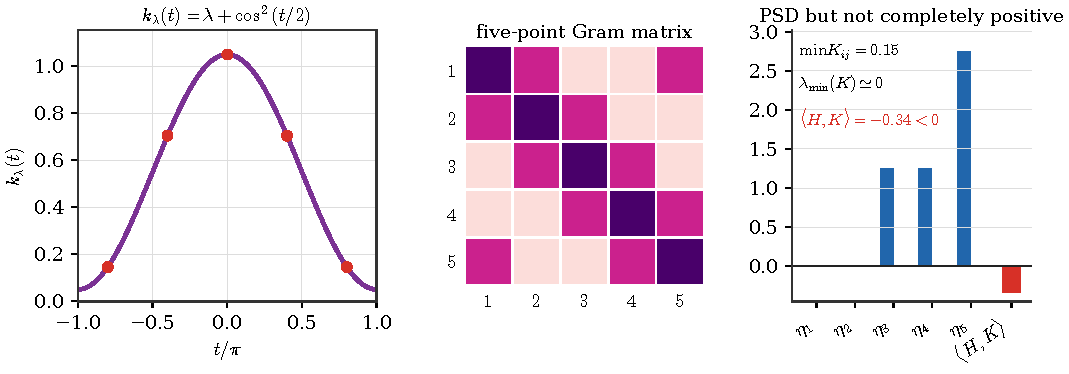
\includegraphics[width=.94\linewidth]{figures/sinkhorn-doubly-positive-counterexample/counterexample.pdf}
\caption{\emph{A doubly positive kernel that is not completely positive.}
The periodic kernel \(k_\lambda(t)=\lambda+\cos^2(t/2)\), with \(\lambda=1/20\), is positive semidefinite and pointwise positive. On five equally spaced points, its Gram matrix is entrywise positive and PSD, but the Horn copositive certificate gives \(\langle H,K\rangle<0\), so this finite restriction is not completely positive and cannot admit a nonnegative Gram factorization.}
\label{fig:sinkhorn-doubly-positive-counterexample}
\end{figure}
\index{Horn matrix}% strictindex
\index{copositive certificate}% strictindex
\index{doubly nonnegative matrix}% strictindex
\index{completely positive matrix}% strictindex
\index{copositive matrix}% strictindex

\index{doubly positive kernel}% strictindex
\index{completely positive kernel}% strictindex

\index{positive!feature map}% strictindex
\index{nonnegative factorization}% strictindex
For a rectangular source--target matrix, Proposition~\ref{prop-cp-kernel-positive-features} is applied to the Gram matrix on the union of the two sampled point sets, after which one extracts the rectangular cross block.

Despite this certification difficulty, completely positive kernels, equivalently positive-sketchable kernels under the assumptions of Proposition~\ref{prop-cp-kernel-positive-features}, enjoy a useful closure algebra. It provides a systematic way to construct new kernels whose low-rank features remain nonnegative.
\begin{prop}[Basic closure of completely positive kernels]
\label{prop-completely-positive-kernel-closure}
\index{completely positive kernel}% strictindex
Let \(k_1,\ldots,k_J\) be completely positive kernels, \(a_1,\ldots,a_J\geq0\), and \((k_\theta)_{\theta\in\Theta}\) a measurable family of completely positive kernels. Whenever they are finite, the sum \(k_{\mathrm{sum}}:=\sum_{j=1}^J a_jk_j\), the product \(k_{\mathrm{prod}}:=\prod_{j=1}^J k_j\), and the mixture \(k_{\mathrm{mix}}:=\int_\Theta k_\theta\,\d\eta(\theta)\), with \(\eta\geq0\), are completely positive. In particular, so is every positive autocorrelation
$k(x,y)=\int g(u-x)g(u-y)\,du$ with $g\geq0$,
and every nonnegative mixture of such kernels.
\end{prop}

\begin{proof}
Restrict the kernels to arbitrary points \(x_1,\ldots,x_n\). If \(K_1=B_1B_1^\top\) and \(K_2=B_2B_2^\top\) with \(B_1,B_2\geq0\), then a nonnegative weighted sum is factored by concatenating the correspondingly rescaled columns. For \(w_{\ell,s}:=(B_1)_{\cdot,\ell}\odot(B_2)_{\cdot,s}\geq0\), one has \(K_1\odot K_2=\sum_{\ell,s}w_{\ell,s}w_{\ell,s}^\top\), so the pointwise product is completely positive. A measurable nonnegative mixture is an integral of matrices in the closed convex cone \(\mathrm{CP}_n\), and therefore remains in that cone. Finally, the autocorrelation formula is itself a scalar positive-feature representation, so its finite Gram matrices are completely positive by the same integral argument.
\end{proof}

For the quadratic cost \(c(x,y)=\norm{x-y}^2\), the Gaussian Gibbs kernel used by Sinkhorn admits the simple positive expectation representation below. It extends to \(e^{-\norm{x-y}^p/\epsilon}\) for \(0<p\leq2\), because radial stable kernels are mixtures of Gaussian kernels. This is the Schoenberg--Bernstein mechanism behind the positive definiteness of radial stable kernels~\cite{schoenberg38,berg84harmonic}. The identity should be distinguished from the bounded-domain positive features of Scetbon and Cuturi~\cite{ScetbonCuturi2020PositiveFeatures}, which were designed to satisfy a relative boundedness condition needed for finite-rank guarantees.

\begin{prop}[Generalized Gaussian positive features]
\label{prop-gaussian-positive-features}
\index{generalized Gaussian kernel}% strictindex
\index{positive!random features}% strictindex
Let \(0<p\leq2\), \(\epsilon>0\), and
	$k_{p,\epsilon}(x,y) = \exp\pa{-\frac{\norm{x-y}^p}{\epsilon}}$ for $x,y\in\RR^d$.
Set \(a=p/2\), let \(S_a\) be the positive \(a\)-stable random variable normalized by
$\EE\pa{e^{-tS_a}}=e^{-t^a}$ for $t\geq0$,
and draw independently \(\Lambda=\epsilon^{-1/a}S_a\) and \(Z\sim\Gaussian(0,\Id_d)\).
For any \(x_0\in\RR^d\), define the positive feature
\[
	\phi_{p,\epsilon}(x;\Lambda,Z)
	:=
	\exp\pa{
		\sqrt{2\Lambda}\dotp{Z}{x-x_0}
		-2\Lambda\norm{x-x_0}^2
	}.
\]
Then \(k_{p,\epsilon}(x,y)=\EE[\phi_{p,\epsilon}(x;\Lambda,Z)\phi_{p,\epsilon}(y;\Lambda,Z)]\), so \(k_{p,\epsilon}\) is completely positive. For i.i.d.\ copies \((\Lambda_\ell,Z_\ell)_{\ell=1}^r\), define the positive sketching features \(\varphi_\ell(x)=r^{-1/2}\phi_{p,\epsilon}(x;\Lambda_\ell,Z_\ell)\), for \(1\leq\ell\leq r\).
They satisfy \(\varphi_\ell\geq0\) and \(\EE[\sum_{\ell=1}^r\varphi_\ell(x)\varphi_\ell(y)]=k_{p,\epsilon}(x,y)\). For \(p=2\), one has \(S_1=1\) almost surely and \(\Lambda=1/\epsilon\), hence
\[
	\phi_{2,\epsilon}(x;Z)
	=
	\exp\pa{
		\sqrt{\frac{2}{\epsilon}}\dotp{Z}{x-x_0}
		-\frac{2}{\epsilon}\norm{x-x_0}^2
	}.
\]
\end{prop}

\begin{proof}
The stable-law normalization gives
$\EE e^{-t\Lambda} = \exp\pa{-\frac{t^a}{\epsilon}}$,
while the Gaussian moment-generating function gives \(\EE_Z[\phi_{p,\epsilon}(x;\Lambda,Z)\phi_{p,\epsilon}(y;\Lambda,Z)]=e^{-\Lambda\norm{x-y}^2}\) conditionally on \(\Lambda\).
Taking \(t=\norm{x-y}^2\) in the first identity proves the feature formula. The Monte Carlo statement follows by averaging independent copies.
\end{proof}

The representation in Proposition~\ref{prop-gaussian-positive-features} is unbiased but its naive Monte-Carlo average need not concentrate. Indeed, writing $u=x-x_0$, $v=y-x_0$, and $F_{x,y}=\phi_{p,\epsilon}(x;\Lambda,Z)\phi_{p,\epsilon}(y;\Lambda,Z)$, a second Gaussian-moment calculation gives
\[
	\EE_Z[F_{x,y}^2\mid\Lambda]
	=
	\exp(8\Lambda\dotp{u}{v}).
\]
At $x=y\neq x_0$, this is $\exp(8\Lambda\norm{u}^2)$. For $0<p<2$, the positive stable mixing variable has no positive exponential moment, so the second moment is infinite; for $p=2$, it grows as $\exp(8\norm{u}^2/\epsilon)$. Thus Proposition~\ref{prop-sinkhorn-sketch-positive-guarantee} does not apply to these raw features, and unbiasedness plus an $O((n+m)r)$ sweep does not provide an end-to-end rank--accuracy guarantee. The localized construction of~\cite{ScetbonCuturi2020PositiveFeatures}, or another controlled approximation scheme, is needed for such a conclusion.

\begin{rem}[The range \(0<p\leq2\)]
\index{positive!random features}% strictindex
The restriction \(0<p\leq2\) is essential. Schoenberg's theorem says that \(x\mapsto e^{-\gamma\norm{x}^p}\) is positive definite on every Euclidean space precisely in this range. For \(p>2\), the generalized Gaussian kernel is not positive definite in general: there are finite Euclidean point clouds for which the Gram matrix has a negative eigenvalue. Thus no universal positive-feature factorization of the above type should be expected. Constants in the cost, such as using \(\norm{x-y}^p/p\), are absorbed by rescaling \(\epsilon\).
\end{rem}
\index{generalized Gaussian kernel}% strictindex
\index{Schoenberg theorem}% strictindex
\index{positive!random features}% strictindex


\paragraph{Positive sketches for Sinkhorn.}
\index{positive!sketch}% strictindex
\index{Gibbs!kernel!sketching}% strictindex
For the \(p\)-power cost \(c_p(x,y)=\norm{x-y}^p\), with \(0<p\leq2\), let
\[
	K_{i,j}=k_{p,\epsilon}(x_i,y_j)
	=\exp\pa{-\frac{\norm{x_i-y_j}^p}{\epsilon}}.
\]
For \(p\geq1\), this is the usual \(p\)-Wasserstein power cost; for \(0<p<1\), it is simply a concave power transport cost. The factor \(1/p\), often used in \(\Wass_p^p\), only rescales \(\epsilon\). Using the sketching features \(\varphi_\ell\) of Proposition~\ref{prop-gaussian-positive-features}, define directly \((\Phi_X)_{i,\ell}=\varphi_\ell(x_i)\) and \((\Phi_Y)_{j,\ell}=\varphi_\ell(y_j)\).
Proposition~\ref{prop-gaussian-positive-features} gives \(K_r:=\Phi_X\Phi_Y^\top\geq0\) entrywise and \(\EE[K_r]=K\). Sinkhorn applied to \(K_r\) uses only products by the two feature matrices, and its plan is represented as
\[
	P_r
	=
	\diag(u)\Phi_X\Phi_Y^\top\diag(v)
	=
	LR^\top,
	\qquad
	L=\diag(u)\Phi_X,
	\quad
	R=\diag(v)\Phi_Y.
\]
The factorization therefore gives $O((n+m)r)$ arithmetic per sweep for every realized sketch, but the preceding moment calculation shows that the raw Monte-Carlo rank required for accuracy is uncontrolled. This algebraic route is complementary to worst-case near-linear Sinkhorn analyses~\cite{altschuler2017near}, low-rank Gaussian-kernel approximations for quadratic transport~\cite{AltschulerBachRudiWeed2018QuadraticTransport}, and factored-coupling models in which the coupling itself is constrained to have low rank~\cite{scetbon2021lowrank}.
\index{positive!random features}% strictindex
\index{entropic!plan}% strictindex
\index{low-rank!coupling}% strictindex

Figure~\ref{fig:sinkhorn-positive-feature-sketching} uses deterministic Gauss--Hermite quadrature for the \(p=2\) feature identity. It illustrates that positive low-rank factors preserve the marginal constraints after scaling but can remain inaccurate in the plan and in logarithmic cost even at moderate rank. For $r=40$, the retained diagnostics give a plan $\ell^1$ error of about $0.735$ and a reference-plan-weighted log-kernel RMSE of about $48.9$; the panel should therefore be read as a distortion study, not as an accuracy certificate.

\begin{figure}[H]
\centering
\begin{tabular}{cccc}

\includegraphics[width=.22\linewidth]{figures/sinkhorn-positive-feature-sketching/exact.pdf} &
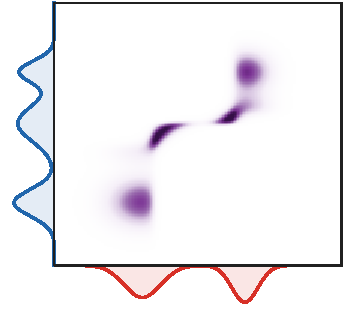
\includegraphics[width=.22\linewidth]{figures/sinkhorn-positive-feature-sketching/rank-040.pdf} &
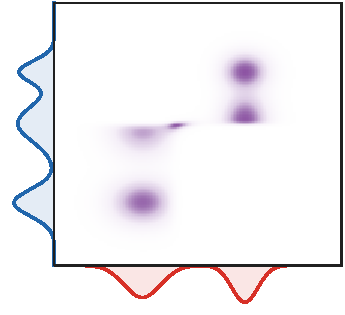
\includegraphics[width=.22\linewidth]{figures/sinkhorn-positive-feature-sketching/rank-010.pdf} &
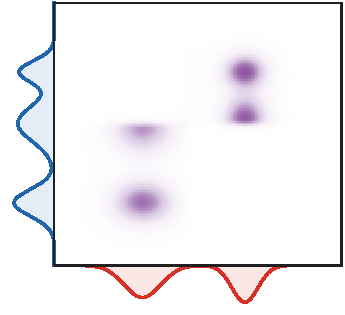
\includegraphics[width=.22\linewidth]{figures/sinkhorn-positive-feature-sketching/rank-003.pdf} \\[-.15em]
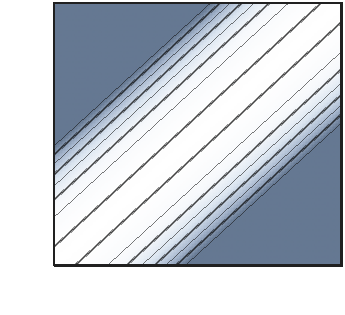
\includegraphics[width=.22\linewidth]{figures/sinkhorn-positive-feature-sketching/cost-exact.pdf} &
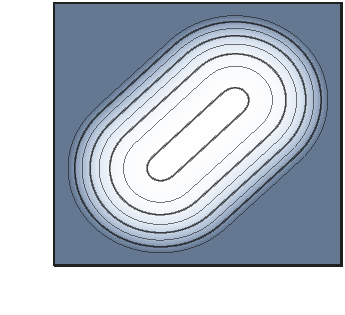
\includegraphics[width=.22\linewidth]{figures/sinkhorn-positive-feature-sketching/cost-rank-040.pdf} &
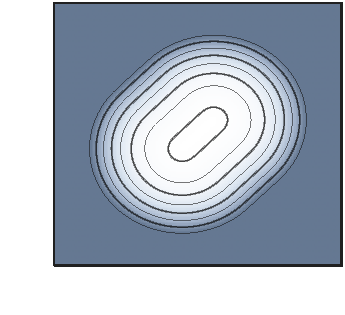
\includegraphics[width=.22\linewidth]{figures/sinkhorn-positive-feature-sketching/cost-rank-010.pdf} &
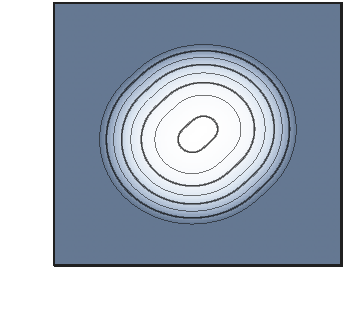
\includegraphics[width=.22\linewidth]{figures/sinkhorn-positive-feature-sketching/cost-rank-003.pdf} \\[-.2em]
exact dense kernel & positive sketch, \(r=40\) & positive sketch, \(r=10\) & positive sketch, \(r=3\)
\end{tabular}
\caption{\emph{Positive-feature sketches can preserve marginals while distorting transport geometry.}
The top row shows entropic couplings between one-dimensional Gaussian mixtures; every sketched plan is rescaled to the prescribed marginals. The bottom row displays \(-\epsilon\log (K_r)_{i,j}\) with black level sets, compared with the exact quadratic cost in the first column. The logarithm floors kernel entries at $10^{-300}$, and the common color display is capped at the $70$th percentile of the exact cost. Even rank $40$ has substantial plan and log-kernel error; ranks $10$ and $3$ further blur the geometry. Deterministic Gaussian quadrature is used for reproducibility.}
\label{fig:sinkhorn-positive-feature-sketching}
\end{figure}

\paragraph{Connection with linear time attention.}
\index{linear!attention}% strictindex
\index{kernel!attention}% strictindex
The same algebra appears in transformer attention, studied later from a continuous-depth transport viewpoint in Section~\ref{sec-transformer-depth-evolution}. A softmax attention matrix has entries proportional to \(\exp(\dotp{q_i}{k_j})\). Feature-based linear attention replaces this positive kernel by \(\phi(q_i)^\top\phi(k_j)\) and, whenever the denominator is positive, computes the normalized output as
\[
	y_i
	=
	\frac{\phi(q_i)^\top\sum_j\phi(k_j)v_j}
	{\phi(q_i)^\top\sum_j\phi(k_j)},
\]
without forming the full attention matrix~\cite{Katharopoulos2020LinearAttention,Choromanski2021Performer}. Linformer instead projects the sequence dimension, while Nystr\"omformer reconstructs attention from landmarks; these are related low-rank strategies but not instances of the same positive-feature identity~\cite{Wang2020Linformer,Xiong2021Nystromformer}. Sinkhorn sketching is the transport analogue of the feature route: replace the Gibbs matrix by a positive factorization, keep only the scaling vectors and feature factors, and control the approximation in the logarithmic scale relevant to entropic potentials. The transport case is more constrained because the approximate kernel is reused inside nonlinear normalizations until both prescribed marginals are reached.
\index{transformer}% strictindex
\index{attention!linear}% strictindex
\index{softmax attention}% strictindex
